% Präambel
\documentclass[%
fontsize=12pt,					% Schriftgröße
paper=a4,						% Papierformat
twoside=false, 					% einseitiges (false) oder zweiseitiges (true) Dokument
listof=totoc, 					% Tabellen- und Abbildungsverzeichnis ins Inhaltsverzeichnis
bibliography=totoc,				% Literaturverzeichnis ins Inhaltsverzeichnis aufnehmen
titlepage, 						% Titlepage-Umgebung statt \maketitle
headsepline, 					% horizontale Linie unter Kolumnentitel
%abstracton,					% Überschrift beim Abstract einschalten, Abstract muss dazu in {abstract}-Umgebung stehen
DIV=12,							% Satzspiegeleinstellung, 12 ist Standar bei KOMA
BCOR=6mm,						% Bindekorrektur, die den Seitenspiegel um 3mm nach rechts verschiebt,
cleardoublepage=empty,			% Stil einer leeren eingefügten Seite bei Kapitelwechsel
parskip,							% Absatzabstand bei Absatzwechsel einfügen
ngerman
]{scrbook}			
\usepackage{float}
\usepackage{tabularx}
\usepackage{booktabs}
\usepackage[setspace=false]{scrhack}
\usepackage[utf8]{inputenc} 	% ermöglicht die direkte Eingabe von Umlauten
\usepackage[T1]{fontenc} 		% Ausgabe aller zeichen in einer T1-Codierung (wichtig für die Ausgabe von Umlauten!)
\usepackage{babel} 	% deutsche Trennungsregeln und Übersetzung der festcodierten Überschriften
\renewcaptionname{ngerman}{\contentsname}{Inhaltsverzeichnis}
\renewcaptionname{ngerman}{\bibname}{Literaturverzeichnis}
\setlength{\parindent}{0ex} 	% bei neuem Abschnitt nicht einrücken
%------
% Folgende Einstellungen entsprechen den Vorgaben der Leitlinien
\usepackage[onehalfspacing]{setspace}
% Ende Leitlinien
%------
%------
% Folgende Einstellungen sind bei größeren Arbeiten mit viel Text zu empfehlen.
% Hierbei oben DIV=16 einstellen und Zeile \usepackage[onehalfspacing]{setspace} auskommentieren.
%\linespread{1.2}\selectfont     % Zeilenabstand erhöhen - größere Werte als 1.2 nicht verwenden!!
% Ende Einstellung große Arbeiten mit viel Text.
%------

\newcommand{\lowrule}{%
	\leavevmode \kern.06em\vbox{\hrule width.5em}}

\usepackage{siunitx}			% Vereinfachte Eingabe von Einheiten in Formeln
\sisetup{
	number-unit-product = \;,
	inter-unit-product = \:,
	exponent-product = \cdot,
	output-decimal-marker = {,}
}

\usepackage{graphicx}  			% Einbinden von Grafiken erlauben
\usepackage[format=hang,		% Formatierungen von Unter- / Überschriften
font=normal,
labelfont=bf,
justification=RaggedRight,
singlelinecheck=true,
aboveskip=1mm
]{caption}

\usepackage[backend=biber, %% Hilfsprogramm "biber" beim Compilieren nutzen (statt "biblatex" oder "bibtex")
style=alphabetic, %% Zitierstil (siehe Dokumentation)
natbib=true, %% Bereitstellen von natbib-kompatiblen Zitierkommandos
hyperref=true, %% hyperref-Paket verwenden, um Links zu erstellen
]{biblatex}
\setcounter{biburllcpenalty}{7000}
\setcounter{biburlucpenalty}{8000}
\addbibresource{literature/literatur1.bib} %% Einbinden der bib-Datei. Endung .bib unbedingt ergänzen
%\addbibresource{literature/literatur2.bib} %% Einbinden mehrerer bib-Dateien mit zusätzlichem \addbibresource - Befehl

\usepackage[normalem]{ulem}
\usepackage{csquotes}
\usepackage{comment}


% Folgende Zeilen sind auszukommentieren, falls runde Klammern und ein vgl. bei Zitaten erscheinen sollen.
%\makeatletter
%\renewcommand{\@cite}[2]{(vgl. {#1\if@tempswa , #2\fi})} 
%\renewcommand{\@biblabel}[1]{(#1)}
%\makeatother

\usepackage{pdfpages}

\usepackage{enumitem}			% Erlaubt Änderung der Nummerierung in der Umgebung enumerate

\usepackage{amsmath}			% Ergänzungen für Formeln
\usepackage{textcomp} 			% zum Einsatz von Eurozeichen u. a. Symbolen
\usepackage{eurosym}			% bessere Darstellung Euro-Symbol mit \euro

\usepackage[					% Einstellunge Paket hyperref
hyperfootnotes=false,			% im pfd-Output Fußnoten nicht verlinken
hidelinks						% Entfernen von farbigen Umrandungen der Links
]{hyperref}

\usepackage{makeidx}			% Paket zur Erstellung eines Index
\usepackage[toc]{glossaries}			% Paket zur Erstellung eines Glossars
\newglossaryentry{gls:glossar}
{
	name=Glossar,
	description={Als Glossar wird eine Liste von ausgewählten Begriffen bezeichnet, denen eine jeweilige Erläuterung zugeordnet ist. Ein Glossar wird, sofern gewünscht, im Anhang des Dokuments hinzugefügt.}
}
\usepackage[intoc]{nomencl} 			% zur Erstellung des Abkürzungsberzeichnisses

\usepackage[					% Einstellungen für Fußnoten
bottom,							% Ausrichtung unten
multiple,						% Trennung durch Seperator bei mehreren Fußnoten
hang,
marginal
]{footmisc}

\usepackage{calc}				% Paket zum Berechnen von Längen z.B. 0.8\linewidth

\usepackage{xcolor} 			% einfache Verwendung von Farben in nahezu allen Farbmodellen

\usepackage{listings}			% Darstellung von Quellcode mit den Umgebungen {lstlisting}, \lstinline und \lstinputlisting
\lstset{literate=				% Damit können Umlaute innerhalb Listings geschrieben werden
	{Ö}{{\"O}}1
	{Ä}{{\"A}}1
	{Ü}{{\"U}}1
	{ß}{{\ss}}1
	{ü}{{\"u}}1
	{ä}{{\"a}}1
	{ö}{{\"o}}1
}
\usepackage{listingsutf8}

\lstdefinelanguage{json}{
	basicstyle=\ttfamily\footnotesize,
	breaklines=true,
	literate=
	*{0}{{{\color{black}0}}}{1}
	{1}{{{\color{black}1}}}{1}
	{2}{{{\color{black}2}}}{1}
	{3}{{{\color{black}3}}}{1}
	{4}{{{\color{black}4}}}{1}
	{5}{{{\color{black}5}}}{1}
	{6}{{{\color{black}6}}}{1}
	{7}{{{\color{black}7}}}{1}
	{8}{{{\color{black}8}}}{1}
	{9}{{{\color{black}9}}}{1}
	{:}{{{\color{black}:}}}{1}
	{,}{{{\color{black},}}}{1}
	{"}{{{\color{black}"}}}{1},
}

\definecolor{mygreen}{rgb}{0,0.6,0}
\definecolor{mygray}{rgb}{0.5,0.5,0.5}
\definecolor{mymauve}{rgb}{0.58,0,0.82}
\lstset{ %
	backgroundcolor=\color{white},   % choose the background color; you must add \usepackage{color} or \usepackage{xcolor}; should come as last argument
	basicstyle=\footnotesize,        % the size of the fonts that are used for the code
	breakatwhitespace=false,         % sets if automatic breaks should only happen at whitespace
	breaklines=true,                 % sets automatic line breaking
	captionpos=t,                    % sets the caption-position to (b) bottom or (t) top
	commentstyle=\color{mygreen},    % comment style
	deletekeywords={...},            % if you want to delete keywords from the given language
	escapeinside={\%*}{*)},          % if you want to add LaTeX within your code
	escapeinside={(*@}{@*)},
	extendedchars=true,              % lets you use non-ASCII characters; for 8-bits encodings only, does not work with UTF-8
	frame=none,	                   	% "single" adds a frame around the code; "none"
	keepspaces=true,                 % keeps spaces in text, useful for keeping indentation of code (possibly needs columns=flexible)
	keywordstyle=\color{blue},       % keyword style
	language=[LaTeX]TeX,             % the language of the code
	morekeywords={*,nomenclature},   % if you want to add more keywords to the set
	numbers=left,                    % where to put the line-numbers; possible values are (none, left, right)
	numbersep=5pt,                   % how far the line-numbers are from the code
	numberstyle=\tiny\color{mygray}, % the style that is used for the line-numbers
	rulecolor=\color{black},         % if not set, the frame-color may be changed on line-breaks within not-black text (e.g. comments (green here))
	showspaces=false,                % show spaces everywhere adding particular underscores; it overrides 'showstringspaces'
	showstringspaces=false,          % underline spaces within strings only
	showtabs=false,                  % show tabs within strings adding particular underscores
	stepnumber=1,                    % the step between two line-numbers. If it's 1, each line will be numbered
	stringstyle=\color{mymauve},     % string literal style
	tabsize=2,	                   % sets default tabsize to 2 spaces
	title=\lstname                   % show the filename of files included with \lstinputlisting; also try caption instead of title
}

% -----------------------------------------------------------------------------------------------------------------
% Zum Aktualisieren des Abkürzungsverzeichnisses (Nomenklatur) bitte auf der Kommandozeile folgenden Befehl aufrufen :
% makeindex <Dateiname>.nlo -s nomencl.ist -o <Dateiname>.nls
% Oder besser: Kann in TexStudio unter Tools-Benutzer als Shortlink angelegt werden
% Konfiguration unter: Optionen-Erzeugen-Benutzerbefehle: makeindex -s nomencl.ist -t %.nlg -o %.nls %.nlo
% -----------------------------------------------------------------------------------------------------------------

% Hier die persönlichen Daten eingeben:

\newcommand{\titel}{Implementierung eines Tracking Systems für Produkte auf einer Fertigungskette}
\newcommand{\arbeit}{Studienarbeit T3\lowrule 3101}
\newcommand{\studiengang}{Embedded Systems}
\newcommand{\autor}{Kilian Röper}
\newcommand{\bearbeitungszeitraum}{01.10.2024 - 15.07.2025}
\newcommand{\matrikelnr}{5928177}
\newcommand{\kurs}{TSA22}
\newcommand{\abgabe}{\today}
\newcommand{\betreuerfirma}{Markus Wengle}

\newcommand{\jahr}{2025}			% für Angabe im Copyright-Vermerk der Titelseite

% Folgende Zeilen definieren Abkürzungen, um Befehle schneller eingeben zu können
\newcommand{\ua}{\mbox{u.\,a.\ }}
\newcommand{\zB}{\mbox{z.\,B.\ }}
\newcommand{\bs}{$\backslash$}
\newcommand*\diff{\mathop{}\!\mathrm{d}}	% Differentialzeichen
\newcommand*\Diff[1]{\mathop{}\!\mathrm{d^#1}} % Differentialzeichen höherer Ableitung
\newcommand*\jj{\mathop{}\!\mathrm{j}}	% Komplexe Zahl j

% Folgende Zeilen weden benötigt, um Tikz und PGF-Plot-Grafiken einzubinden
\usepackage{pgfplots}
\usepackage{pgfplotstable}
\pgfplotsset{compat=newest,width=0.6\linewidth}
\usepgfplotslibrary{smithchart}
\usepackage{tikz}						% Tikz sollte nach Listings Pakete geladen werden.
\usetikzlibrary{arrows}
\usetikzlibrary{arrows.meta, positioning, shapes.geometric, calc}

\tikzstyle{component} = [rectangle, rounded corners, minimum width=2.8cm, minimum height=1cm,text centered, draw=black, fill=blue!10]
\tikzstyle{mqtt} = [->, thick, dashed, color=blue]
\tikzstyle{wired} = [->, thick, color=black]
\tikzstyle{legendbox} = [rectangle, draw=none, fill=none, font=\small]


\hyphenation{Schrift-ar-ten}

%\BeforeClosingMainAux{% siehe KOMA-Script-Anleitung
%\addcontentsline{toc}{chapter}{\indexname}\stepcounter{page}
%}

\makeindex						% Indexverzeichnis erstellen
\makenomenclature				% Abkürzungsverzeichnis erstellen
%\makeglossaries

% -------------------------------------------------------------------------------------------
%                     Beginn des Dokumenteninhalts
% -------------------------------------------------------------------------------------------
\begin{document}
\let\texteuro\euro						% Eingabe \texteuro, € oder \euro erzeugt gleiches Ergebnis
\setcounter{secnumdepth}{3}				% Nummerierungstiefe fürs Inhaltsverzeichnis
\setcounter{tocdepth}{3}
\sffamily								% für die Titelei serifenlose Schrift verwenden

% ------------------------------ Titelei -----------------------------------------------------

\thispagestyle{plain}
\hypersetup{pageanchor=false}
\begin{titlepage}
\enlargethispage{4.0cm}
\sffamily 								% Serifenlose Grundschrift für die Titelseite einstellen

\parbox{0.5\linewidth}{
\begin{flushleft}
% Hier ggf. ein Logo der Firma
\end{flushleft}
}
\parbox{0.5\linewidth}{
\begin{flushright}
	
\includegraphics[width=0.4\linewidth]{images/DHBW_d_R_FN_46mm_4c}\\[5ex]
\end{flushright}
}
				

\begin{center}

{\fontsize{20.74pt}{24pt}\selectfont
\textbf{\titel}\\[1.5ex]}
{\fontsize{17pt}{20pt}\selectfont
\textbf{\arbeit}\\[2ex]}
{\fontsize{14pt}{17pt}\selectfont
Studiengang \studiengang\\[2ex]}
{\fontsize{12pt}{14pt}\selectfont
Duale Hochschule Baden-Württemberg Ravensburg, Campus Friedrichshafen\\[5ex]
von\\[1ex]
\autor\\[15ex]}


\end{center}

\begin{flushleft}
{\fontsize{12pt}{14pt}\selectfont
\begin{tabular}{ll}
Abgabedatum:					& \quad \abgabe \\
Bearbeitungszeitraum:		   	& \quad \bearbeitungszeitraum   \\ 
Matrikelnummer: 			& \quad \matrikelnr \\ 
Kurs: 							& \quad \kurs \\
Betreuerin / Betreuer:  & \quad \betreuerfirma \\ % Betreuerin / Betreuer der Arbeit
\end{tabular}
}
\end{flushleft}
%%%%% Nachfolgende Zeilen einkommentieren, wenn Copyrightvermerk gewünscht ist
%\begin{flushleft}
%{\fontsize{11pt}{13pt}\selectfont
%Copyrightvermerk:\\
%Dieses Werk einschließlich seiner Teile ist \textbf{urheberrechtlich geschützt}. Jede Verwertung außerhalb der engen Grenzen des Urheberrechtgesetzes ist ohne Zustimmung des Autors unzulässig und strafbar. Das gilt insbesondere für Vervielfältigungen, Übersetzungen, Mikroverfilmungen sowie die Einspeicherung und Verarbeitung in elektronischen Systemen.
%}
%\end{flushleft}
%\begin{flushright}
%{\fontsize{11pt}{13pt}\selectfont \copyright{} \jahr }
%\end{flushright}
\end{titlepage}

\ifthenelse{\boolean{@twoside}}{%
	\cleardoublepage
}{%
	\clearpage
}%

\hypersetup{pageanchor=true}
 				% erzeugt die Titelseite
\pagenumbering{roman}					% kleine, römische Seitenzahlen für Titelei
%% Ggf. folgende Zeile auskommentieren, falls der Sperrvermerk gewünscht ist.
%\chapter*{Sperrvermerk} %*-Variante sorgt dafür, das der Sperrvermerk nicht im Inhaltsverzeichnis auftaucht
%gemäß Ziffer 1.1.14 der Anlage 1 zu §§ 3, 4 und 5  der Studien- und Prüfungsordnung für die Bachelorstudiengänge im Studienbereich Technik der Dualen Hochschule Baden-Württemberg vom 29.09.2017 in der Fassung vom 24.07.2023:
%
%Der Inhalt dieser Arbeit darf weder als Ganzes noch in Auszügen Personen außerhalb des Prüfungsprozesses und des Evaluationsverfahrens zugänglich gemacht werden, sofern keine anders lautende Genehmigung vom Dualen Partner vorliegt.
%
%Musterstadt, den \today \\[4ex]
%
%\rule[-0.2cm]{5cm}{0.5pt} \\
%
%\textsc{\autor} \\[10ex]

\chapter*{Erklärung} %*-Variante sorgt dafür, dass die Erklärung nicht im Inhaltsverzeichnis auftaucht

gemäß Ziffer 1.1.14 der Anlage 1 zu §§ 3, 4 und 5  der Studien- und Prüfungsordnung für die Bachelorstudiengänge im Studienbereich Technik der Dualen Hochschule Baden-Württemberg vom 29.09.2017 in der Fassung vom 24.07.2023.

Ich versichere hiermit, dass ich meine \arbeit\ mit dem Thema:

\begin{quote}
	\textit{\titel} % -\textit{ \untertitel }
\end{quote}

selbstständig verfasst und keine anderen als die angegebenen Quellen und Hilfsmittel benutzt habe. Ich versichere zudem, dass die eingereichte elektronische Fassung mit der gedruckten Fassung übereinstimmt.\\[6ex]

Friedrichshafen, den \today \\[1ex]

\rule[-0.2cm]{5cm}{0.5pt} \\

\autor \\[10ex]

\rmfamily

\thispagestyle{empty}

 				% Einbinden der eidestattlichen Erklärung
\chapter*{Kurzfassung} %*-Variante sorgt dafür, das Abstract nicht im Inhaltsverzeichnis auftaucht

Die Lernfabrik produziert teilautomatisiert über eine Fertigungskette verschiedene Produkte. Zur Verbesserung der Steuerung, Nachverfolgbarkeit und Dokumentation soll ein System entwickelt werden, das die Position der Produkte mittels NFC-Technologie erfasst und die entsprechenden Daten an ein Manufacturing Execution System (MES) übermittelt. Während geeignete NFC-Tags bereits identifiziert wurden, muss die restliche Systemarchitektur standortspezifisch konzipiert, implementiert und getestet werden.

Ziel dieser Arbeit ist die Entwicklung eines industrietauglichen Systems zur positionsbasierten Produktverfolgung innerhalb der Fertigung. Die erfassten Informationen sollen in Echtzeit an ein vorhandenes System übertragen und dort visualisiert werden.

Zur Entwicklung der Systemarchitektur kamen klassische ingenieurwissenschaftliche Methoden zum Einsatz. Der Fokus lag auf einem kosteneffizienten, störungstoleranten und modular erweiterbaren Aufbau der Hardware- und Softwarekomponenten.

Die Arbeit mündete in einem vollständigen Systementwurf zur produktionsbegleitenden Datenerfassung über NFC. Realisiert wurde ein Prototyp bestehend aus dezentralen Erfassungseinheiten und einer zentralen Steuereinheit, die eine Schnittstelle zum MES bereitstellt. Neben der Hardware wurden die erforderlichen Softwarekomponenten zur Datenübertragung und -visualisierung sowie eine technische Dokumentation für zukünftige Erweiterungen erstellt.

\clearpage

\chapter*{Abstract} %*-Variante sorgt dafür, das Abstract nicht im Inhaltsverzeichnis auftaucht

The learning factory produces various products semi-automatically via a production chain. To improve control, traceability, and documentation, a system is to be developed that records the position of the products using NFC technology and transmits the corresponding data to a Manufacturing Execution System (MES). While suitable NFC tags have already been identified, the remaining system architecture must be designed, implemented, and tested site-specifically.

The goal of this work is to develop an industrial-grade system for position-based product tracking within production. The recorded information is to be transmitted in real time to an existing system and visualized there.

Classical engineering methods were used to develop the system architecture. The focus was on a cost-effective, fault-tolerant, and modularly expandable design of the hardware and software components.

The work culminated in a complete system design for production-related data acquisition via NFC. A prototype was realized consisting of decentralized acquisition units and a central control unit that provides an interface to the MES. In addition to the hardware, the necessary software components for data transmission and visualization as well as technical documentation for future extensions were created.

\clearpage   			% Einbinden des Abstracts

\tableofcontents						% Erzeugen des Inhalsverzeichnisses

\clearpage

% --------------------------------------------------------------------------------------------
%                    Inhalt der Bachelorarbeit
%---------------------------------------------------------------------------------------------
\pagenumbering{arabic}					% arabische Seitenzahlen für den Hauptteil

\rmfamily

\chapter{Einleitung}
\label{cha:Einleitung}

Mit der zunehmenden Automatisierung industrieller Produktionsprozesse wächst der Bedarf an intelligenten Systemen, die eine lückenlose Nachverfolgbarkeit und effiziente Steuerung ermöglichen.
Besonders in vernetzten Fertigungsumgebungen, wie sie im Kontext von Industrie-4.0 realisiert werden, spielt die automatische Identifikation von Produkten entlang der Fertigungskette eine zentrale Rolle. Zum Einsatz kommen dafür verschiedene Technologien - von optischer Erkennung bis hin zu RFID und NFC (Near Field Communication).

Die Lernfabrik der DHBW bietet eine reale, teilautomatisierte Fertigungsumgebung, in der solche Konzepte unter praxisnahen Bedingungen erprobt werden können. Aktuell fehlt jedoch ein System zur durchgängigen Identifikation und Nachverfolgung von Produkten innerhalb der Fertigungslinie. Dies erschwert nicht nur die Prozessüberwachung, sondern limitiert auch Möglichkeiten zur Datenanalyse, Optimierung und Dokumentation.

Ziel dieser Arbeit ist die Entwicklung eines Systems, das die Position und Identität von Produkten während des Fertigungsprozesses mit Hilfe von NFC-Sensoren automatisch erfasst. Zusätzlich soll es möglich sein Informationen automatisch auf die NFC-Tag zu schreiben. Die erfassten Daten werden an ein bestehendes Manufacturing Execution System (MES) übermittelt und dort zur Visualisierung bereitgestellt. Darüber hinaus sollen die von den NFC-Sensoren erfassten Informationen genutzt werden, um den logischen Ablauf des Bandumlaufsystems zu steuern. Hierfür ist ein Kommunikationsmechanismus zwischen den einzelnen Bandumlaufstationen und den NFC-Sensoren zu entwerfen. Im Rahmen dieser Arbeit wird eine geeignete Systemarchitektur für die Hard- und Softwarekomponenten konzipiert, implementiert und evaluiert.

Die zentrale Fragestellung der Arbeit lautet:
\begin{quote}
	\textit{Wie kann ein robustes, kosteneffizientes und erweiterbares Trackingsystem für Produkte in einer bestehenden Fertigungsumgebung mithilfe von NFC-Technologie gestaltet und in ein MES integriert werden?}
\end{quote}


Zur Beantwortung dieser Frage werden klassische ingenieurwissenschaftliche Methoden wie Anforderungsanalyse, Systementwurf, prototypische Umsetzung und Validierung angewendet. Neben der technischen Umsetzung liegt ein besonderes Augenmerk auf der industriellen Tauglichkeit sowie der zukünftigen Erweiterbarkeit des Systems.

Die Arbeit gliedert sich wie folgt:  
Kapitel~2 beschreibt die theoretischen und technischen Grundlagen der verwendeten Technologien. Kapitel~3 analysiert die Anforderungen an das System und erläutert das methodische Vorgehen. Kapitel~4 enthält den Entwurf der Systemarchitektur sowie die Darstellung und Auswertung der Ergebnisse. Abschließend fasst Kapitel~5 die wesentlichen Erkenntnisse zusammen und gibt einen Ausblick auf mögliche Weiterentwicklungen.

\chapter{Grundlagen}
\label{cha:Grundlagen}


Dieses Kapitel stellt die theoretischen und technischen Grundlagen bereit, die für das Verständnis und die Umsetzung der im weiteren Verlauf beschriebenen Konzepte und Lösungen erforderlich sind. Dazu gehören sowohl technologische Aspekte – wie die Funktionsweise von RFID/NFC-Systemen oder des MQTT-Protokolls – als auch methodische Grundlagen im Bereich der Kommunikation und Steuerung verteilter Systeme.

Ziel ist es, ein solides Fundament zu schaffen, auf dem die spätere Systemkonzeption und Implementierung aufbauen kann. Die hier dargestellten Inhalte stehen daher in engem Zusammenhang mit den folgenden Kapiteln und werden dort zur Anwendung gebracht – beispielsweise bei der Auswahl geeigneter Kommunikationsprotokolle, Hardwarekomponenten oder der Integration in die Gesamtarchitektur des Systems.

\section{RFID und NFC-Technologie}
\label{sec:nfc}

Near Field Communication (NFC) ist eine auf der RFID-Technologie (radio-frequency identification) basierende drahtlose Kommunikationstechnologie, die speziell für die Kommunikation über kurze Distanzen von wenigen Zentimetern entwickelt wurde. Sie ermöglicht den kontaktlosen Datenaustausch zwischen zwei NFC-fähigen Geräten, wobei ein Gerät aktiv (z.B. ein Smartphone) und das andere passiv (z.B. ein NFC-Tag) sein kann. Wesentliche Unterschiede zwischen RFID und NFC sind in \autoref{tab:rfid_vs_nfc} festgehalten. 

\begin{table}[H]
	\centering
	\caption{Vergleich zwischen RFID und NFC}
	\label{tab:rfid_vs_nfc}
	\begin{tabular}{|p{4cm}|p{4.5cm}|p{4.5cm}|}
		\hline
		\textbf{Eigenschaft} & \textbf{RFID} & \textbf{NFC} \\
		\hline
		Frequenzbereich & Verschiedene Bereiche: LF (125–134 kHz), HF (13,56 MHz), UHF (860–960 MHz) & HF (13,56 MHz) \\
		\hline
		Kommunikations- Richtung & In der Regel unidirektional (Reader zu Tag) & Bidirektional (Peer-to-Peer möglich) \\
		\hline
		Reichweite & Bis zu mehreren Metern (je nach Frequenz) & Typisch 0–10 cm \\
		\hline
		Datenrate & Abhängig vom Standard, z.B. bis zu 640 kbit/s (UHF) & Bis zu 424 kbit/s \\
		\hline
		Typische Anwendungen & Lagerlogistik, Zutrittskontrolle, Tierkennzeichnung, Supply Chain & Mobile Payment, Geräteverbindung, Zugangskontrolle im Konsumerbereich \\
		\hline
		Standardisierung & ISO/IEC 18000, ISO/IEC 14443, 15693 usw. & ISO/IEC 14443, ISO/IEC 18092, NFC Forum Spezifikationen \\
		\hline
		Interoperabilität & Eingeschränkt (herstellerspezifisch, viele Standards) & Hoch (interoperabel durch NFC Forum Vorgaben) \\
		\hline
	\end{tabular}
\end{table}

NFC arbeitet in einem Frequenzbereich von 13,56MHz und ermöglicht Datenraten von bis zu 424kbit/s. Der wichtigste Unterschied zu klassischen RFID-Systemen liegt in der bidirektionalen Kommunikation: Während RFID meist eine unidirektionale Leser-Tag-Kommunikation darstellt, ermöglicht NFC einen wechselseitigen Datenaustausch. Die typische maximale Reichweite beträgt etwa 10cm, wodurch eine gezielte, sichere Interaktion gewährleistet wird \autocite[Seite 47 Tabelle 3.6]{finkenzeller2023}. 

Die Technologie kommt u.a. bei mobiler Bezahlung (z.B. Apple Pay), elektronischen Zugangssystemen, öffentlichen Verkehrsmitteln sowie bei der schnellen Geräteverbindung (z.B. Bluetooth-Kopplung) zum Einsatz. In dieser Arbeit wird die Technologie zum Austausch von Informationen zwischen NFC-Readern und Tags an einer Fertigungskette verwendet. In \autoref{cha:vorgehen} wird genauer darauf eingegangen wie hierfür die Integration in die Gesamtarchitektur erfolgt. Zur Implementierung von NFC-basierten Funktionen stehen für Embedded-Systeme verschiedene Softwarebibliotheken zur Verfügung (vgl. \ref{sec:systementwurf}). Diese ermöglichen etwa das Auslesen und Schreiben von NFC-Tags oder das Initiieren von Peer-to-Peer-Verbindungen.


\section{Das MQTT-Protokoll}
\label{sec:mqtt}

MQTT (Message Queuing  Telemetry Transport)  ist ein Client-Server-Publish/Subscribe-Nachrichtentransportprotokoll. Es ist leichtgewichtig, offen, einfach und leicht zu implementieren. Diese Eigenschaften prädestinieren es für den Einsatz in vielen Situationen, auch in eingeschränkten Umgebungen, wie z. B. für die Kommunikation im Machine-to-Machine- (M2M) und Internet of Things-Kontext (IoT), wo ein geringer Code-Footprint erforderlich ist und/oder die Netzwerkbandbreite knapp ist \cite[Abstract]{oasis_mqtt_spec}.

Das Protokoll läuft über TCP/IP oder andere Netzwerkprotokolle, die geordnete, verlustfreie und bidirektionale Verbindungen ermöglichen. Zu seinen Funktionen gehören:

\begin{itemize}

\item Verwendung des Publish/Subscribe-Nachrichtenmusters, das eine One-to-Many-Nachrichtenverteilung und die Entkopplung von Anwendungen ermöglicht.

\item Drei Dienstqualitäten für die Nachrichtenübermittlung

\item Ein Nachrichtentransport, der vom Inhalt der Nutzlast unabhängig ist.

\item Geringer Transportaufwand und minimierter Protokollaustausch reduzieren den Netzwerkverkehr.

\item Ein Mechanismus zur Benachrichtigung interessierter Parteien bei einer ungewöhnlichen Verbindungsunterbrechung.

\end{itemize}


Das Protokoll wurde mit dem Ziel entwickelt, eine möglichst leichtgewichtige und ressourcenschonende Kommunikation zu ermöglichen, insbesondere über Netzwerke mit hoher Latenz oder geringer Bandbreite. Im Vergleich zu traditionellen Client-Server-Modellen verwendet MQTT das Publish-/Subscribe-Prinzip, das eine entkoppelte Kommunikation erlaubt. In dieser Arbeit wird MQTT als Kommunikationsschicht zwischen Sensoren und einem Raspberry Pi eingesetzt [\ref{sec:systementwurf}].

Im Folgenden werden die zentralen Konzepte des Protokolls näher erläutert: das Publish-/Subscribe-Prinzip, die Rollen von Client und Broker sowie die verschiedenen Quality-of-Service-Stufen.

\subsection*{Publish-/Subscribe-Prinzip}
\label{sub:pub_sub_mqtt}

MQTT basiert auf einem Publish-/Subscribe-Modell. Ein \emph{Publisher} sendet Nachrichten an ein bestimmtes \emph{Topic}, ohne dabei explizit anzugeben, wer diese Nachrichten empfangen soll. Topics dienen in MQTT als hierarchisches Adressierungsschema zur Organisation von Nachrichten. Sie sind UTF-8-kodierte Strings, die durch Schrägstriche ("/") strukturiert sind, z.B. \texttt{sensor/temperatur/wohnzimmer}. Ein \emph{Subscriber} hingegen abonniert ein oder mehrere Topics und erhält automatisch alle Nachrichten, die zu diesen Topics veröffentlicht werden [\autoref{fig:mqtt_pubsub}].

\subsection*{Client und Broker}

Die zentrale Vermittlungsinstanz in diesem Modell ist der sogenannte \emph{Broker}. Er empfängt alle vom Publisher gesendeten Nachrichten und leitet sie an die entsprechenden Subscriber weiter. Jeder Teilnehmer in einem MQTT-Netzwerk ist ein \emph{Client}, unabhängig davon, ob er Nachrichten veröffentlicht oder abonniert. Der Broker übernimmt die vollständige Verwaltung der Kommunikation: Er sorgt dafür, dass Nachrichten zuverlässig und effizient verteilt werden, ohne dass sich Publisher und Subscriber gegenseitig kennen oder direkt kommunizieren müssen. Diese Architektur entkoppelt Sender und Empfänger sowohl räumlich als auch zeitlich \cite[Abschnitt 4.7]{oasis_mqtt_spec} [\autoref{fig:mqtt_pubsub}].

\begin{figure}[H]
	\centering
	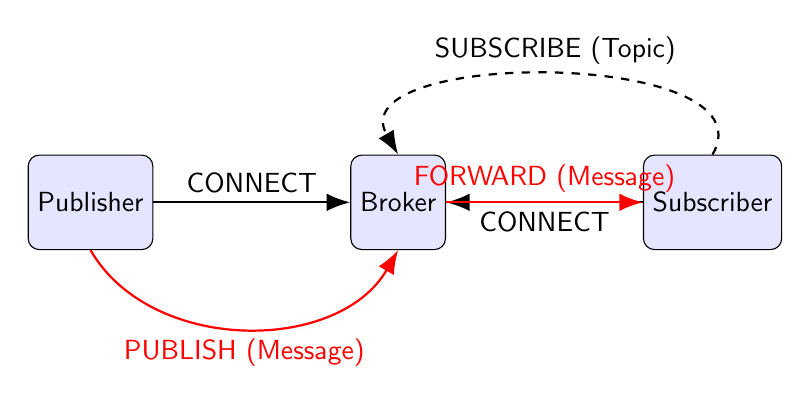
\begin{tikzpicture}[
		node distance=2.5cm and 2.5cm,
		every node/.style={font=\sffamily},
		process/.style={rectangle, draw, rounded corners, minimum height=1.2cm, text centered, fill=blue!10},
		arrow/.style={-{Latex[length=3mm]}, thick}
		]
		
		% Nodes
		\node[process] (publisher) {Publisher};
		\node[process, right=of publisher] (broker) {Broker};
		\node[process, right=of broker] (subscriber) {Subscriber};
		
		% Connection arrows
		\draw[arrow] (publisher) -- node[above] {CONNECT} (broker);
		\draw[arrow] (subscriber) -- node[below] {CONNECT} (broker);
		
		\draw[arrow, dashed] (subscriber.north) to[out=60,in=120] node[above] {SUBSCRIBE (Topic)} (broker.north);
		
		\draw[arrow, thick, red] (publisher.south) to[out=-60,in=-120] node[below] {PUBLISH (Message)} (broker.south);
		
		\draw[arrow, thick, red] (broker.east) -- node[above] {FORWARD (Message)} (subscriber.west);
		
	\end{tikzpicture}
	\caption{Ablauf des MQTT Publish-/Subscribe-Verfahrens mit Verbindungsaufbau}
	\label{fig:mqtt_pubsub}
\end{figure}

\subsection*{Quality of Service (QoS)}

MQTT bietet drei verschiedene Stufen der Nachrichten-Zustellungssicherheit (Quality of Service), die je nach Anwendungsfall gewählt werden können:

\begin{itemize}
	\item \textbf{QoS 0} – ''höchstens einmal'': Nachrichten werden nach bestem Wissen und Gewissen der Betriebsumgebung zugestellt. Nachrichtenverlust kann auftreten. Diese Stufe kann beispielsweise bei Umgebungssensordaten eingesetzt werden, bei denen der Verlust eines einzelnen Messwerts unerheblich ist, da der nächste kurz darauf veröffentlicht wird.
	\item \textbf{QoS 1} – ''mindestens einmal'': Nachrichten werden garantiert ankommen, es können aber Duplikate auftreten.
	\item \textbf{QoS 2} – ''genau einmal'': Nachrichten werden garantiert genau einmal ankommen. Diese Stufe kann beispielsweise bei Abrechnungssystemen eingesetzt werden, bei denen doppelte oder verlorene Nachrichten zu falschen Gebühren führen können. \cite[Abschnitt 4.3]{oasis_mqtt_spec}.
\end{itemize}

\section{Node-Red - Eine Steuerungs- und Visualisierungssoftware}
\label{sec:mes}

Node-RED ist ein von IBM entwickeltes Open-Source-Tool zur visuellen Programmierung, das auf Node.js basiert. Es ermöglicht die Erstellung von Anwendungen durch das Verbinden sogenannter Nodes in einem webbasierten Editor. Ursprünglich für das Internet der Dinge (IoT) konzipiert, findet Node-RED heute Anwendung in Bereichen wie Heimautomation, industrieller Steuerung und Datenintegration \autocite{nodered_official}. 

Die zentrale Einheit in Node-RED ist der Flow, eine Abfolge von miteinander verbundenen Nodes, die Daten verarbeiten und weiterleiten. Jede Node erfüllt dabei eine spezifische Funktion, z.B. das Empfangen von Daten, deren Verarbeitung oder das Senden von Ergebnissen. Die Kommunikation zwischen den Nodes erfolgt über standardisierte Nachrichtenobjekte im JSON-Format, die typischerweise folgende Eigenschaften enthalten:

\begin{itemize}
	
	\item msgid: Eine eindeutige Kennung der Nachricht
	
	\item payload: Die eigentlichen Nutzdaten
	
	\item topic: Ein optionaler Themenbezeichner zur Kategorisierung	

\end{itemize}

Diese Struktur bildet die Grundlage für die Datenverarbeitung in Node-RED. Ein beispielhafter Flow ist in \autoref{fig:node_red_flow} abgebildet.

\begin{figure}[H]
	\centering
	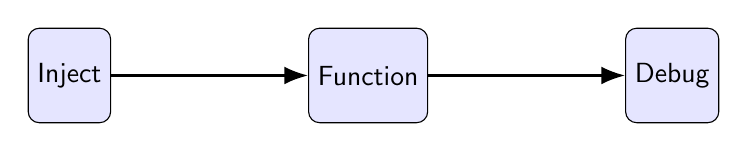
\begin{tikzpicture}[
		node distance=2.5cm and 2.5cm,
		every node/.style={font=\sffamily},
		process/.style={rectangle, draw, rounded corners, minimum height=1.2cm, text centered, fill=blue!10},
		arrow/.style={-{Latex[length=3mm]}, thick}
		]
		% Nodes
		\node[process] (inject) {Inject};
		\node[process, right=of inject] (function) {Function};
		\node[process, right=of function] (debug) {Debug};
		
		% Arrows
		\draw[arrow] (inject) -- (function);
		\draw[arrow] (function) -- (debug);
	\end{tikzpicture}
	\caption{Ein einfacher Node-RED-Flow: Inject → Function → Debug}
	\label{fig:node_red_flow}
\end{figure}

Ein \emph{Inject}-Node erzeugt eine Nachricht mit einem definierten \emph{Payload}. Ein \emph{Function}-Node verarbeitet die Nachricht, beispielsweise durch Anwendung einer JavaScript-Funktion. Der \emph{Debug}-Node gibt das Ergebnis im Debug-Fenster des Editors aus. Solche Flows ermöglichen eine schnelle und intuitive Entwicklung von Anwendungen, ohne tiefgreifende Programmierkenntnisse.

Darüber hinaus bietet Node-RED die Möglichkeit, grafische Benutzeroberflächen mithilfe des sogenannten \emph{Node-RED Dashboards} zu erstellen. Diese Oberflächen können in einem separaten Browser-Fenster aufgerufen werden und eignen sich insbesondere zur Echtzeitvisualisierung von Prozessdaten. In  \autoref{cha:umsetzung} wird diese Funktionalität exemplarisch genutzt, um eine interaktive Darstellung des Bandumlaufsystems zu realisieren und Benutzereingaben zur Steuerung zu ermöglichen.

\section{Speicherprogrammierbare Steuerungen (SPS)}
\label{sec:sps}

Speicherprogrammierbare Steuerungen (SPS) sind spezialisierte, industrielle Recheneinheiten zur Automatisierung technischer Prozesse. Sie ersetzen konventionelle, fest verdrahtete Steuerungssysteme und bieten eine flexible, softwarebasierte Möglichkeit zur Realisierung komplexer Ablaufsteuerungen. SPS-Systeme sind in nahezu allen Bereichen der Industrieautomation zu finden – von einfachen Förderbändern bis hin zu hochkomplexen Produktionslinien \autocite{siemensSCEGuide}.

\subsection{Aufbau einer SPS}

Eine SPS besteht aus mehreren funktionalen Einheiten: einer zentralen Recheneinheit (CPU), digitalen oder analogen Ein- und Ausgabemodulen (I/O), einer Spannungsversorgung sowie optionalen Kommunikationsschnittstellen und Programmierschnittstellen. Das folgende Diagramm zeigt den grundsätzlichen Aufbau:

\begin{figure}[H]
	\centering
	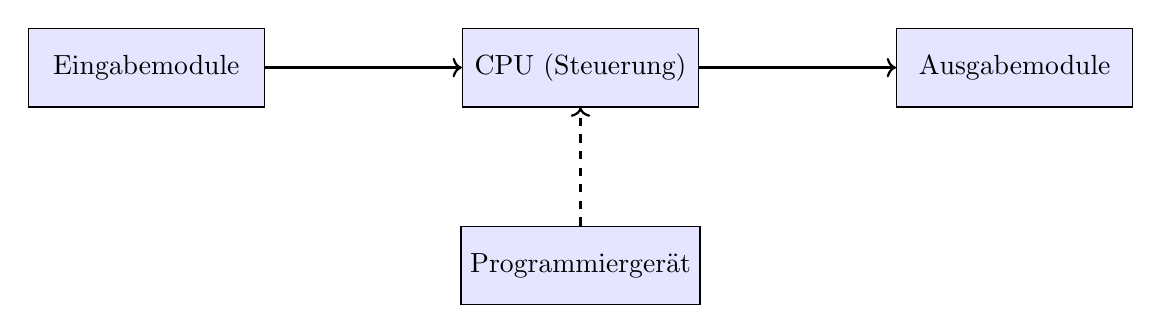
\begin{tikzpicture}[
		block/.style={draw, rectangle, minimum height=1cm, minimum width=3cm, text centered, fill=blue!10},
		line/.style={->, thick}
		]
		\node[block] (input) {Eingabemodule};
		\node[block, right=2.5cm of input] (cpu) {CPU (Steuerung)};
		\node[block, right=2.5cm of cpu] (output) {Ausgabemodule};
		\node[block, below=1.5cm of cpu] (pg) {Programmiergerät};
		
		\draw[line] (input) -- (cpu);
		\draw[line] (cpu) -- (output);
		\draw[line, dashed] (pg) -- (cpu);
	\end{tikzpicture}
	\caption{Schematischer Aufbau einer SPS}
	\label{fig:sps_aufbau}
\end{figure}

\subsection{Funktionsweise: Der SPS-Zyklus}

Die Arbeitsweise einer SPS basiert auf dem EVA-Prinzip (Eingabe – Verarbeitung – Ausgabe). Dabei werden zyklisch alle Eingänge gelesen, der Steuerungsalgorithmus (z.B. in Form eines SPS-Programms) verarbeitet und anschließend die entsprechenden Ausgänge gesetzt. Dieser Ablauf, auch \textit{SPS-Zyklus} genannt, wiederholt sich kontinuierlich.

\begin{figure}[H]
	\centering
	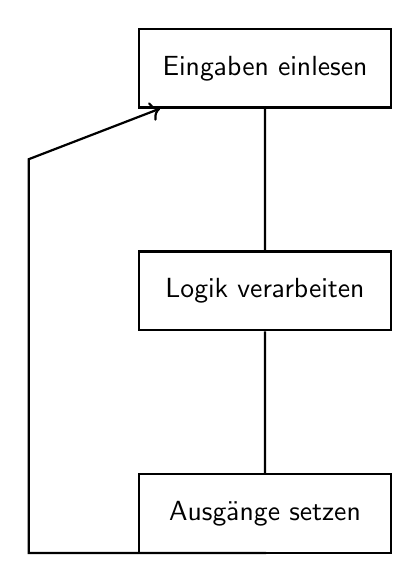
\begin{tikzpicture}[node distance=1.8cm, every node/.style={draw, rectangle, minimum width=3.2cm, minimum height=1cm, font=\sffamily}, ->, thick]
		\node (e) {Eingaben einlesen};
		\node[below=of e] (v) {Logik verarbeiten};
		\node[below=of v] (a) {Ausgänge setzen};
		\draw (e) -- (v) -- (a) -- ++(0,-0.5) -- ++(-3,0) -- ++(0,5) -- (e);
	\end{tikzpicture}
	\caption{Zyklus einer SPS-Steuerung}
	\label{fig:sps_zyklus}
\end{figure}

\subsection{Programmiersprachen nach IEC 61131-3}

Die Norm IEC 61131-3 definiert fünf standardisierte Programmiersprachen für SPS:

\begin{itemize}
	\item \textbf{KOP (Kontaktplan)} – grafische Darstellung mit Relaislogik
	\item \textbf{FUP (Funktionsplan)} – logische Gatterstruktur (ähnlich wie digitale Schaltungen)
	\item \textbf{AWL (Anweisungsliste)} – Assembler-ähnlich
	\item \textbf{ST (Structured Text)} – textbasierte Hochsprache (ähnlich Pascal)
	\item \textbf{SFC (Sequential Function Chart)} – Ablaufsteuerungen mit Schritten und Transitionen
\end{itemize}

Ein Beispiel in \textit{Structured Text (ST)} zeigt eine einfache UND-Verknüpfung zweier Eingänge:

\begin{lstlisting}[language=Pascal, caption={Beispielprogramm in Structured Text}, label={lst:st_example}]
	IF Eingang1 = TRUE AND Eingang2 = FALSE THEN
	Ausgang := TRUE;
	ELSE
	Ausgang := FALSE;
	END_IF;
\end{lstlisting}

\section{Serial Peripheral Protocoll (SPI)}
\label{sec:spi}



\chapter{Konzeptentwurf}
\label{cha:vorgehen}

\subsection{Anforderungsanalyse mittels Requirements Engineering}

\subsection{Hardwarebewertung mithilfe einer Nutzwertanalyse}

\subsection{Systementwurf basierend auf den gewählten Komponenten}

Je nach Art der Arbeit kann diese Kapitelüberschrift auch \glqq Konzeptentwurf\grqq~lauten.

Beschreibung der Ausgangssituation und des Themenumfelds. Ggf. wird darauf eingegangen, welche Randbedingungen und Einflüsse zu beachten sind.

Anforderungsanalyse und Anforderungsdefinition, nach Möglichkeit strukturiert, um zu einem späteren Zeitpunkt die Anforderungen nachvollziehbar verifizieren zu können.

Herleitung einer Lösung (einer Methodik, eines experimentellen Aufbaus oder von unterschiedlichen Konzepten), Lösungsbewertung und bewusste Wahl des gewählten Vorgehens. An dieser Stelle ist auch auf die Zuverlässigkeit einer Methodik oder auf die Genauigkeit von Untersuchungen einzugehen. Die Überlegungen sollen dazu helfen, mit der angestrebten Lösung die gestellten Anforderungen zu erfüllen, um schließlich die Ziele der Arbeit erreichen zu können.

Bei einer Gegenüberstellung von verschiedenen Lösungsansätzen kann z.~B. eine Nutzwertanalyse helfen. Dabei sind nicht nur z.~B. die Funktion, Leistungsfähigkeit, Umsetzbarkeit und Nutzbarkeit, sondern auch z.~B. wirtschaftliche Aspekte, wie Stück-, Entwicklungskosten oder Ressourcenverbrauch zu berücksichtigen. Sehr bedeutend sind auch Aspekte der Nachhaltigkeit unter Betrachtung des gesamten Lebenszyklus einer erarbeiteten Lösung.

Sowohl bei der Anforderungsdefinition, als auch bei der Lösungsfindung gibt es eine große Anzahl an verschiedenen Methoden. Eine kleine Auswahl ist in der folgenden Aufzählung zu finden.

\begin{itemize}
\item Anforderungsdefinition mithilfe des Requirements Engineering  \autocite{Pohl.2021}
\item Systems Engineering Ansatz \autocite{Schluter.2023}
\item Agile Entwicklungsmethodiken \autocite{Cohn.2010, Martin.2020, Wirdemann.2022}
\item Klassische Bewertungsverfahren \autocite{Breiing.1997, Zangemeister.2014}
\end{itemize}

Ziel dieses Kapitels ist, dass auf Basis von umfassend und genau formulierten Anforderungen (ggf. auch Nicht-Zielen) eine Lösungsvielfalt erarbeitet wird, welche anschließend strukturiert bewertet wird, um eine fundierte Begründung für die angestrebte Art der Umsetzung herzuleiten.
\chapter{Umsetzung der Softwarearchitektur}
\label{cha:umsetzung}
\section{Softwaredesign auf den Mikrocontrollern}
\label{sec:Node-MCU}

\subsection{Softwarearchitektur und Designtools}

Die Softwarearchitektur auf den eingesetzten ESP8266-Mikrocontrollern wurde mit der Arduino-IDE angefertigt. Sie gliedert sich in zwei Hauptkomponenten:

\begin{itemize}
	\item \textbf{Setup-Funktion:} Verantwortlich für die Überprüfung der Kommunikationsfähigkeit der erstellten Kommunikations-Objekte.
	\item \textbf{Loop-Funktion:} Verwaltet den Zugriff auf den MQTT-Client, den PN532-Leser sowie das Auslesen und Schreiben der Speicherblöcke.
\end{itemize}


\subsection{Systemstart und Initialisierung}

Beim Systemstart werden zunächst globale Variablen und Objektinstanzen initialisiert, die für die spätere Kommunikation und Datenverarbeitung erforderlich sind [siehe \autoref{lst:init_globals}]. Dazu zählen:

\begin{itemize}
	\item Ein WiFi-Objekt, das die Netzwerkverbindung herstellt und damit die Grundlage für die MQTT-Kommunikation bildet.
	\item Ein SPI-Objekt, das die serielle Verbindung zum PN532-NFC-Sensor über das SPI-Protokoll ermöglicht.
\end{itemize}

Basierend auf diesen Kommunikationsschnittstellen werden zwei zentrale Objekte global angelegt:

\begin{itemize}
	\item Ein NFC-Objekt, das über das SPI-Objekt mit dem PN532-Sensor kommuniziert.
	\item Ein MQTT-Objekt, das über das WiFi-Objekt mit dem MQTT-Broker verbunden wird.
\end{itemize}

Zusätzlich werden globale Variablen definiert, die während der Laufzeit von verschiedenen Programmteilen gelesen und verändert werden können. Dazu gehören unter anderem:

\begin{itemize}
	\item die UID-Variable, welche die eindeutige Kennung des erfassten NFC-Tags speichert,
	\item sowie die io\_state-Variable, die den aktuellen Verarbeitungszustand an der Station eines Produkts repräsentiert.
\end{itemize}

\newpage

\begin{lstlisting}[language=C, caption={Initialisierung globaler Objekte und Variablen}, label={lst:init_globals}]
	// Globale Kommunikationsobjekte
	// SPI-connection
	PN532_SPI intf(SPI, PN532_SS);
	PN532 nfc = PN532(intf);
	// wifi and mqtt client 
	WiFiClient wifiClient;
	MqttClient mqttClient(wifiClient);
	
	// Globale Zustandsvariablen
	uint8_t uid_data[UID_LENGTH] = {0};
	uint8_t io_state[4] = {0};
\end{lstlisting}


In der Setup-Funktion, die einmalig beim Systemstart ausgeführt wird, werden die Verbindungen mithilfe der zuvor erstellten Objekte erstellt. Das Wifi-Objekt wird mit dem Netzwerk des Raspberry Pi verbunden. Dann kann über das MQTT-Objekt eine Verbindung zu dem Broker hergestellt werden. Mithilfe des NFC-Objekts wird überprüft ob die Verbindung zum PN532-Sensor über SPI hergestellt werden konnte. 

Das MQTT-Objekt wird außerdem dazu genutzt eine Callback-Funktion zu registrieren, mithilfe dieser der Informationsgehalt der empfangenen Nachrichten in die globale Zustands-Variable geschrieben wird. Zuletzt wird das Objekt genutzt, um ein Topic zu abonnieren. An der Werkerassistenzstation wird das Topic ''rfid/assembling\_mcu\_receive'' abonniert [siehe \autoref{lst:mqtt_sub}]. 

\begin{lstlisting}[language=C, caption={Abonnieren des MQTT-Topics in der Setup-Funktion}, label={lst:mqtt_sub}]
	// subscribe to a topic
	mqttClient.subscribe(topic_receive);
\end{lstlisting}

\subsection{Zustandsverarbeitung und Hauptschleife}

Die Hauptschleife folgt auf allen Mikrocontrollern der selben Logik wurde aber jeweils an die individuellen Anforderungen angepasst. Beispielsweise wird an der Werkerassistenzstation die UID eines Tags vergeben werden, falls es noch nicht geschehen ist. Ein Codeausschnitt dieser Station - explizit die Loop-Funktion - ist im Anhang festgehalten [siehe \autoref{lst:assembling_loop}].

Die Hauptschleife prüft kontinuierlich, ob ein NFC-Tag im Lesebereich erkannt wurde [siehe \autoref{fig:flowchart_mcu}]. Wird ein Tag erfasst, so wird die UID gelesen und die relevanten Speicherblöcke geschrieben [siehe \autoref{lst:writing_block}]. Wenn alle Informationen erfolgreich geschrieben wurden, wird eine Nachricht via MQTT mit den neuen Zuständen an den Broker gesendet. 

\begin{lstlisting}[language=C, caption = Funktion zum Schreiben einer Information auf einen Speicherblock am Beispiel der Werkerassistenzstation, label=lst:writing_block]
	success = nfc.mifareultralight_WritePage(ASSEMBLING_BLOCK, io_state_temp);
\end{lstlisting}

Für den Fall, dass eine Nachricht vom Broker empfangen wurde und ein Tag im Empfangsbereich ist, wird die erhaltene Information in den entsprechenden Speicherbereich geschrieben. Das erfordert jedoch, dass ein Tag an einer Station etwas länger verweilt. Diese Zeit wird festgehalten und wenn der Tag dann schließlich entfernt wird, wird eine erneute MQTT-Nachricht gesendet, die über die Weiterfahrt zur nächsten Station informiert. 

Diese Logik wird fortlaufend in einer Schleife durchlaufen.

\tikzstyle{startstop} = [rectangle, rounded corners, minimum width=3cm, minimum height=1cm,text centered, draw=black, fill=gray!20]
\tikzstyle{process} = [rectangle, minimum width=3cm, minimum height=1cm, text centered, draw=black, fill=blue!10]
\tikzstyle{decision} = [diamond, aspect=2, text centered, draw=black, fill=yellow!20, inner sep=1pt]
\tikzstyle{arrow} = [thick,->,>=stealth]


\begin{figure}[H]
	\centering
	\begin{tikzpicture}[node distance=1.5cm]
		
		% Nodes
		% start
		\node (start) [startstop] {Start Loop};
		\node (mqttpoll) [process, below of=start] {MQTT \texttt{poll()} aufrufen};
		\node (readtag) [decision, below of=mqttpoll, yshift=-0.5cm] {Tag erkannt?};
		\node (alreadywritten) [decision, below of=readtag, yshift=-1cm] {Tag bereits beschrieben?};
		\node (handlemsg) [decision, right of=alreadywritten, xshift=5cm] {MQTT-Nachricht erhalten?};
		
		% processes
		\node (writetag) [process, below of=alreadywritten, yshift=-1cm] {Zustand auf Tag schreiben};
		\node (readuid) [process, below of=writetag] {UID prüfen und ggf. zuweisen};
		\node (writetracking) [process, below of=readuid] {Tracking-Status auf Tag schreiben};
		\node (sendmqtt) [process, below of=writetracking] {MQTT-Nachricht an PI senden};
		
		% end
		\node (writetime) [process, below of=handlemsg, yshift=-2.5cm] {Tag-Zeit am Sensor festhalten};
		\node (tagdelay) [decision, below of=writetime, yshift=-1cm] {Länger als 2\,s im Feld?};
		\node (tagdetached) [decision, below of=tagdelay, yshift=-1cm] {Tag entfernt};
		\node (senddetach) [process, below of=tagdetached, yshift=-0.5cm] {MQTT: Statuswechsel an PI senden};
		
		\node (end) [startstop, left of=senddetach, xshift=-5cm] {Loop Ende / neuer Durchlauf};
		
		% Arrows
		% start
		\draw [arrow] (start) -- (mqttpoll);
		\draw [arrow] (mqttpoll) -- (readtag);
		\draw [arrow] (readtag) -- node[anchor= west] {ja} (alreadywritten);
		\draw [arrow] (readtag) -- node[anchor= west] {ja} (handlemsg);
		\draw [arrow] (readtag) -- ++(-3,0) |- node[anchor= north east] {nein} (start);
		\draw [arrow] (alreadywritten) -- node[anchor= east] {nein} (writetag);
		\draw [arrow] (handlemsg) -- node[anchor=south] {ja} (writetag);
		\draw [arrow] (alreadywritten.east) -- node[anchor=west] {ja} (writetime);
		\draw [arrow] (handlemsg) -- node[anchor=south] {nein} (writetime);
		
		% processes
		\draw [arrow] (writetag) -- (readuid);
		\draw [arrow] (readuid) -- (writetracking);
		\draw [arrow] (writetracking) -- (sendmqtt);
		\draw [arrow] (sendmqtt) -- (end);
		
		% dispatch decision
		\draw [arrow] (writetime) -- (tagdelay);
		\draw [arrow] (tagdelay) -- node[anchor=west] {ja} (tagdetached);
		\draw [arrow] (tagdelay) -- node[anchor=west] {nein} (end);
		\draw [arrow] (tagdetached) -- node[anchor=west] {ja} (senddetach);
		\draw [arrow] (tagdetached) -- node[anchor=west] {nein} (end);
		\draw [arrow] (senddetach) -- (end);
	\end{tikzpicture}
	\caption{Ablaufdiagramm der Hauptlogik auf dem Mikrocontroller}
	\label{fig:flowchart_mcu}
\end{figure}

\newpage

\subsection{Kommunikation über MQTT}

Die Kommunikation mit dem Dashboard erfolgt mithilfe eines Raspberry Pi über das MQTT-Protokoll. Jeder Mikrocontroller veröffentlicht Zustandsänderungen auf einem dedizierten Topic wie \texttt{rfid/shelf\_mcu\_send}. Die Daten werden im JSON-Format übertragen [siehe \autoref{lst:mqtt_json}].

\begin{lstlisting}[language=json, caption={Beispiel einer MQTT JSON Nachricht von der Werkerassistenzstation (0x04: zur Schraubstation, 1: iO) (siehe \autoref{tab:tracking_states})}, label={lst:mqtt_json}]
	{
		"uid": "AB CD EF 02",
		"tracking": "0x04",
		"state": "1"
	}
\end{lstlisting}

Werden Daten für ein abonniertes Topic empfangen, wird in die registrierte Callback Funktion [siehe \autoref{lst:mqtt_callback}] gesprungen und der erhaltene neue Zustand wird in die globale Zustands-Variable geschrieben. Zudem wird eine Variable gesetzt mit der dann in der Loop-Funktion erkannt wird, dass eine Nachricht empfangen wurde[siehe \autoref{fig:flowchart_mcu}]. Dadurch kann der neue Zustand, durch Zugriff auf die globale Variable in den Speicher des sich im Erkennungsbereich befindlichen NFC-Tags geschrieben werden. 

\begin{lstlisting}[language=C, caption={Registrierung des Callbacks in der Setup-Funktion}, label={lst:mqtt_callback}]
	// set the message receive callback
	mqttClient.onMessage(onMqttMessage);
\end{lstlisting}

\section{Visualisierung der Prozessdaten in Node-RED}
\label{sec:Node-Red}

\begin{figure}[H]
	\centering
	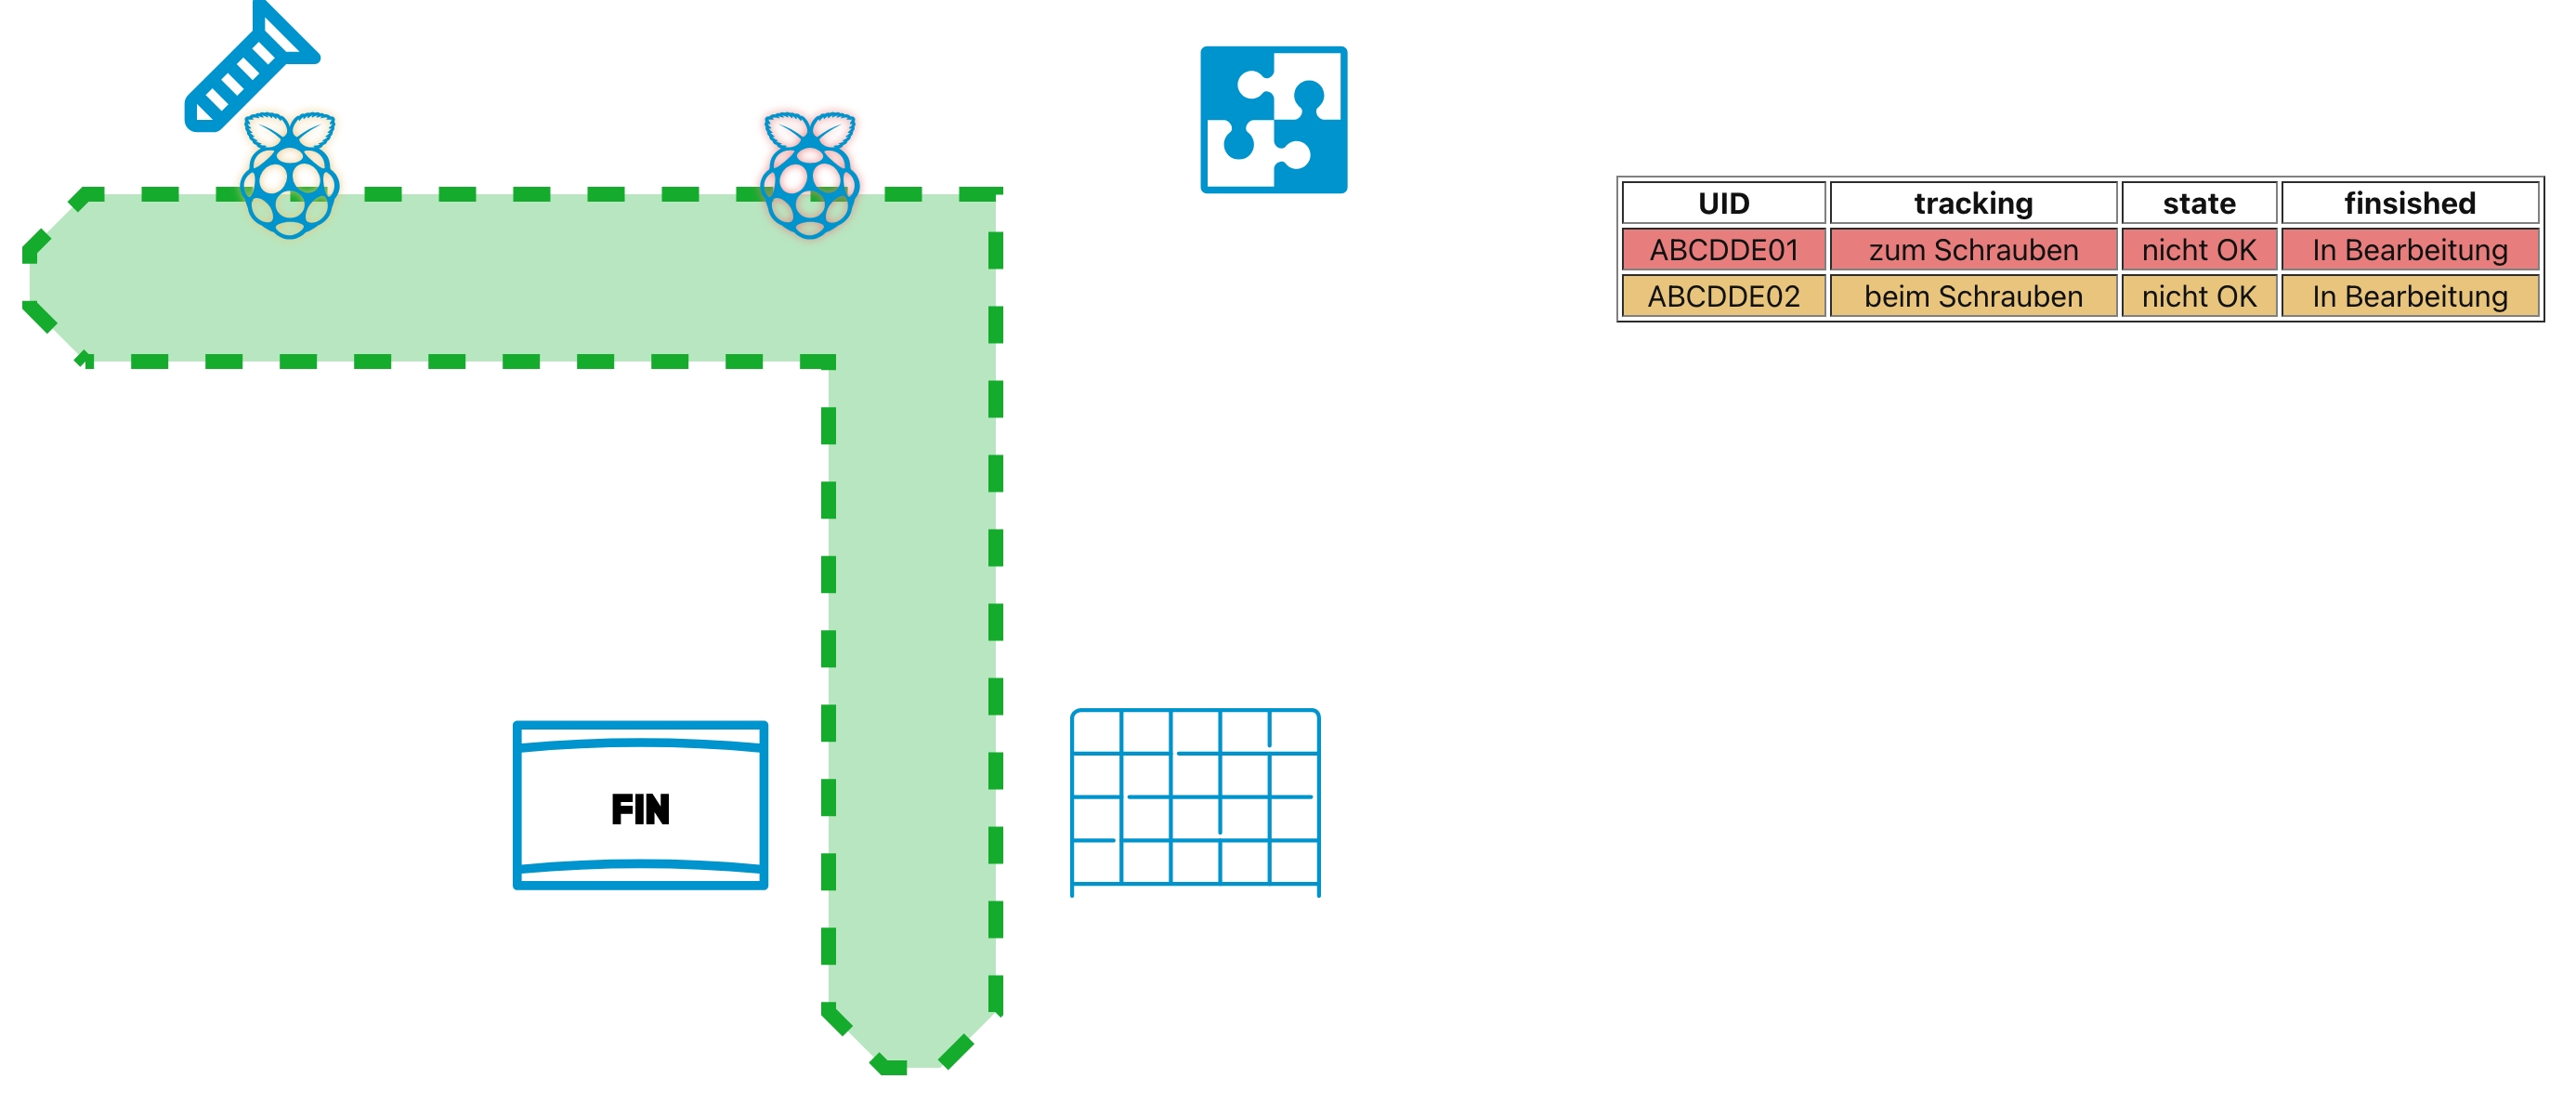
\includegraphics[width=0.8\textwidth]{images/node-red-band.jpeg}
	\caption{Node-RED-Dashboard des NFC-Tracking-Systems}
	\label{fig:dashboard}
\end{figure}

Zur Visualisierung der Produktpositionen und Produktzustände wurde ein interaktives Dashboard mit Node-RED implementiert (siehe \autoref{fig:dashboard}). Dieses Dashboard stellt die vier Stationen geometrisch entsprechend ihrer Anordnung in der Lernfabrik dar. Produkte werden symbolisch als Raspberry-Pi-Icons dargestellt und entlang des virtuellen Förderbands basierend auf ihrem erfassten Tracking-Zustand positioniert.

Die aktuelle Systemübersicht umfasst zwei Hauptkomponenten:
\begin{itemize}
	\item \textbf{Visuelle Darstellung des Förderbands:} Produkte bewegen sich entsprechend ihres Zustands zwischen den Stationen.
	\item \textbf{Tabelle mit Produktinformationen:} Für jedes Produkt wird eine eindeutige UID sowie der aktuelle Tracking-Zustand, der letzte Bearbeitungsstatus und ein Fertigstellungsindikator angezeigt. Die Zeilen sind farblich codiert, um die visuelle Unterscheidbarkeit der Produkte zu erhöhen.
\end{itemize}

\begin{figure}[H]
	\centering
	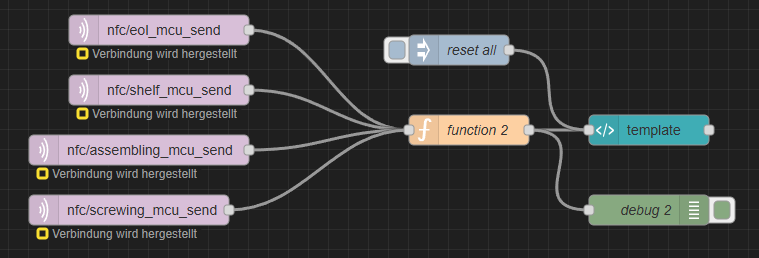
\includegraphics[width=0.8\textwidth]{images/node-red-flow-receive.png}
	\caption{Node-RED-Flow zum Empfang von Nachrichten}
	\label{fig:receive_nodes}
\end{figure}

Node-RED ermöglicht eine visuelle und modulare Abbildung der Prozesslogik. Die Empfangslogik ist in \autoref{fig:receive_nodes} dargestellt. Dabei werden vier verschiedene MQTT-Topics mithilfe des MQTT-In-Nodes abonniert. Diese vier Topics sind die auf denen von den vier Stationen der Zustand gesendet wird. Die empfangenen JSON-Daten werden anschließend von einem Function-Node analysiert. Dieser Node sorgt dafür das die virtuellen Produkte korrekt Positioniert und die Informationen tabellarisch korrekt dargestellt werden. Nach dem Weiterleiten der überarbeiteten Informationen, sorgt der Template-Node für eine korrekte Darstellung im Dashboard. Alle Zugangsinformationen können \autoref{tab:systemkonfiguration} entnommen werden. 

\begin{table}[H]
	\centering
	\caption{Systemkonfiguration Node-RED und MQTT}
	\label{tab:systemkonfiguration}
	\begin{tabular}{ll}
		\toprule
		\textbf{Komponente} & \textbf{Einstellung / Wert} \\
		\midrule
		Node-RED Dashboard Adresse     & \texttt{http://localhost:1880/ui} \\
		MQTT-Broker Adresse            & \texttt{10.42.0.1} (im MQTT-Node)\\
		MQTT-Port                      & \texttt{1883} (im MQTT-Node)\\
		Verbindung                     & Raspberry Pi WiFi Access Point \\
		SSID                           & \texttt{rfid\_ritz\_access\_point} \\
		Passwort                       & \texttt{rfid32\_connect} \\
		Broker-Start                   & Automatisch über Access Point beim \\  & Systemstart des Raspberry Pi\\
		Remote-Zugang zum Raspberry Pi & ritzpi@raspberrypi.local \\
		Username Raspberry Pi 	   	   & ritzpi		\\
		Passwort Raspberry Pi 		   & njkjjm	   \\
		SCP Datenübertragung vom Pi	   & scp ritzpi@raspberrypi.local:~/file.py . \\
		SCP Datenübertragung zum Pi	   & scp ./file.py ritzpi@raspberrypi.local:~ \\
		\bottomrule
	\end{tabular}
\end{table}

Zusätzlich enthält der Flow einen Reset-Node zum Zurücksetzen des Dashboards sowie einen Debug-Node zur Laufzeitanalyse [siehe \autoref{fig:receive_nodes}].

\begin{figure}[H]
	\centering
	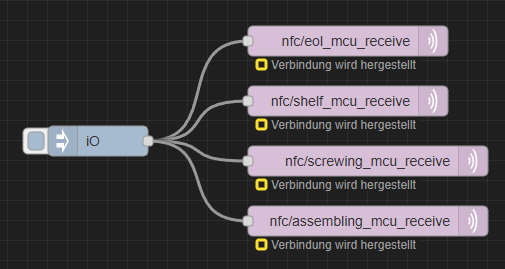
\includegraphics[width=0.8\textwidth]{images/node-red-flow-send.png}
	\caption{Node-RED-Flow zum Senden von Nachrichten an Stationen}
	\label{fig:send_nodes}
\end{figure}

Für Testzwecke wurde ein dedizierter Sende-Flow implementiert (\autoref{fig:send_nodes}). Dieser ermöglicht das manuelle Senden von Zustands-Informationen an die Mikrocontroller an den Stationen über vier weitere MQTT-Topics. Diese haben dieselbe Namenskonvention wie die Empfangs-Topics, enthalten jedoch den Suffix \texttt{mcu\_receive} anstelle von \texttt{mcu\_send}. So kann eine einfache manuelle Steuerung einzelner Produktzustände direkt aus dem Dashboard heraus erfolgen. 

Jeder ESP8266 an einer Station ist zu seinem Topic abonniert und springt in eine Callback-Funktion, um die empfangene MQTT-Nachricht zu verarbeiten und auf einen Tag zu schreiben. Diese Topics können genutzt werden, um den Zustand eines Produkts der an einer Station ermittelt und an die Haupt-SPS weitergeleitet wird, von der SPS aus über MQTT den erhaltenen Zustand weiterzugeben, wodurch das Schreiben vom ESP8266 über den Callback erfolgt. Alle vorhandenen MQTT-Topics sind in \autoref{tab:mqtt_topics} aufgelistet.

Diese abonnierten Topics ermöglichen es die zur Laufzeit am Bandumlaufsystem ermittelten Zustände auf den Tag zu schreiben. Zunächst können die Produktzustände von einer Station an die Haupt-SPS übertragen werden. Von dort wird der Zustand über MQTT weitergeleitet. Der ESP8266 empfängt diesen Zustand auf seinem Topic und schreibt die Info über den Callback-Mechanismus auf den Tag.

\begin{table}[H]
	\centering
	\caption{MQTT-Topics}
	\label{tab:mqtt_topics}
	\begin{tabular}{|c|l|}
		\hline
		\textbf{Topic} & \textbf{Beschreibung} \\ \hline
		$rfid/eol\_mcu\_send$ & Datenübertragung von der EOL-Station zum Broker \\ 
		$rfid/shelf\_mcu\_send$ & Datenübertragung von der Lagerstation zum Broker \\ 
		$rfid/assembling\_mcu\_send$ & Datenübertragung von der Montage-Station zum Broker \\ 
		$rfid/screwing\_mcu\_send$ & Datenübertragung von der Schraubstation zum Broker \\ \hline
		$rfid/eol\_mcu\_receive$ & Datenübertragung vom Broker an die EoL-Station \\ 
		$rfid/shelf\_mcu\_receive$ & Datenübertragung vom Broker an die Lagerstation\\ 
		$rfid/assembling\_mcu\_receive$ & Datenübertragung vom Broker an die Montage-Station\\ 
		$rfid/screwing\_mcu\_receive$ & Datenübertragung vom Broker an die Schraubstation \\ \hline
	\end{tabular}
\end{table}



\chapter{Zusammenfassung}
\label{cha:zusammenfassung}

Fragestellung:
Kann ein robustes, kosteneffizientes und erweiterbares Trackingsystem für Produkte in einer bestehenden Fertigungsumgebung mithilfe von NFC-Technologie gestaltet werden?

Auf zwei bis drei Seiten soll auf folgende Punkte eingegangen werden:

\begin{itemize}
	\item Welches Ziel sollte erreicht werden
	\item Welches Vorgehen wurde gewählt
	\item Was wurde erreicht, zentrale Ergebnisse nennen, am besten quantitative Angaben machen
	\item Konnten die Ergebnisse nach kritischer Bewertung zum Erreichen des Ziels oder zur Problemlösung beitragen
	\item  Ausblick
\end{itemize}

In der Zusammenfassung sind unbedingt klare Aussagen zum Ergebnis der Arbeit zu nennen. Üblicherweise können Ergebnisse nicht nur qualitativ, sondern auch quantitativ benannt werden, z.~B. \glqq \ldots konnte eine Effizienzsteigerung von \SI{12}{\percent} erreicht werden.\grqq~oder \glqq \ldots konnte die Prüfdauer um \SI{2}{\hour} verkürzt werden\grqq.

Die Ergebnisse in der Zusammenfassung sollten selbstverständlich einen Bezug zu den in der Einleitung aufgeführten Fragestellungen und Zielen haben.


% ---- Literaturverzeichnis ----------
\interlinepenalty 10000					% Verhindert einen Umbruch mitten in Literatureinträgen
\printbibliography						% Erstellen des Literaturverzeichnisses
\interlinepenalty 0
\clearpage

% -----Ausgabe aller Verzeichnisse ---
\setlength{\parskip}{0.5\baselineskip}

% Alle Abkürzungen, die in der Arbeit verwendet werden. Die Alphabetische Sortierung übernimmt Latex. Nachfolgend sind Beispiele genannt, welche nach Bedarf angepasst, gelöscht oder ergänzt werden können.
% Die Angaben in der eckigen Klammer werden zur Sortierung der Einträge verwendet. Vor allem bei Formelzeichen hat man sonst das Problem, dass diese möglicherweise nicht wie gewünscht sortiert werden.

% Bei den unten stehenden Formelzeichen ist erläutert, wie explizite Sortierschlüssel über den Inhalt der eckigen Klammer angegeben werden.

% Zum Aktualisieren des Abkürzungsverzeichnisses (Nomenklatur) bitte auf der Kommandozeile folgenden Befehl aufrufen :
% makeindex <Dateiname>.nlo -s nomencl.ist -o <Dateiname>.nls
% Oder besser: Kann in TexStudio unter Tools-Benutzer als Shortlink angelegt werden
% Konfiguration unter: Optionen-Erzeugen-Benutzerbefehle: makeindex -s nomencl.ist -t %.nlg -o %.nls %.nlo

% Allgemeine Abkürzungen %%%%%%%%%%%%%%%%%%%%%%%%%%%%
%\nomenclature[Abb]{Abb.}{Abbildung}
%\nomenclature[bzw]{bzw.}{beziehungsweise}
%\nomenclature[DHBW]{DHBW}{Duale Hochschule Baden-Württemberg}
%\nomenclature[ebd]{ebd.}{ebenda}
%\nomenclaturev[etal]{et al.}{at alii}
%\nomenclature[etc]{etc.}{et cetera}
%\nomenclature[evtl]{evtl.}{eventuell}
%\nomenclature[f]{f.}{folgende Seite}
%\nomenclature[ff]{ff.}{fortfolgende Seiten}
%\nomenclature[ggf]{ggf.}{gegebenenfalls}
%\nomenclature[Hrsg]{Hrsg.}{Herausgeber}
%\nomenclature[Tab]{Tab.}{Tabelle}
%\nomenclature[ua]{u. a.}{unter anderem}
%\nomenclature[usw]{usw.}{und so weiter}
%\nomenclature[vgl]{vgl.}{vergleiche}
%\nomenclature[zB]{z. B.}{zum Beispiel}
%\nomenclaturev[zT]{z. T.}{zum Teil}

% Dateiendungen %%%%%%%%%%%%%%%%%%%%%%%%%%%%%%%%%%%%
%\nomenclature[EMF]{EMF}{Enhanced Metafile}
%\nomenclature[JPG]{JPG}{Joint Photographic Experts Group}
%\nomenclature[KI]{KI}{Künstliche Intelligenz}
%\nomenclature[PDF]{PDF}{Portable Document Format}
%\nomenclature[PNG]{PNG}{Portable Network Graphics}
%\nomenclature[]{XML}{Extensible Markup Language}

% Abkürzungen von Fachbegriffen %%%%%%%%%%%%%%%%%%%%
%\nomenclature[ABS]{ABS}{Antiblockiersystem}
%\nomenclature[ESC]{ESC}{Electronic Stability Control, Fahrdynamikregelung}

% Formelzeichen %%%%%%%%%%%%%%%%%%%%%%%%%%%%%%%%%%%%
%\nomenclature[a]{$a$}{Beschleunigung}
%\nomenclature[F]{$F$}{Kraft}
%\nomenclature[m]{$m$}{Masse}
%\nomenclature[P]{$P$}{Leistung}
%\nomenclature[U]{$U$}{Spannung}
%\nomenclature[R]{$R$}{Widerstand}

% Abkürzungen Studienarbeit

% Kommunikation & Protokolle (p)
\nomenclature[p]{MQTT}{Message Queuing Telemetry Transport}
\nomenclature[p]{SPI}{Serial Peripheral Interface}
\nomenclature[p]{TCP}{Transmission Control Protocol}
\nomenclature[p]{I2C}{Inter-Integrated Circuit}
\nomenclature[p]{QoS}{Quality of Service}
\nomenclature[p]{JSON}{JavaScript Object Notation}
\nomenclature[p]{UTF-8}{8-Bit Unicode Transformation Format}
\nomenclature[p]{WiFi}{Wireless Fidelity}

% Automatisierung / SPS (s)
\nomenclature[s]{SPS}{Speicherprogrammierbare Steuerung}
\nomenclature[s]{TIA Portal}{Totally Integrated Automation Portal}
\nomenclature[s]{FUP}{Funktionsplan}
\nomenclature[s]{KOP}{Kontaktplan}
\nomenclature[s]{AWL}{Anweisungsliste}
\nomenclature[s]{ST}{Structured Text}
\nomenclature[s]{SFC}{Sequential Function Chart}
\nomenclature[s]{MES}{Manufacturing Execution System}
\nomenclature[s]{EVA}{Eingabe Verarbeitung Ausgabe}
\nomenclature[s]{EoL}{End of Line}

% Kommunikation / Schnittstellen / Busse (k)
\nomenclature[k]{MOSI}{Master Out Slave In}
\nomenclature[k]{MISO}{Master In Slave Out}
\nomenclature[k]{SCLK}{Serial Clock}
\nomenclature[k]{SS/CS}{Slave Select / Chip Select}
\nomenclature[k]{CPOL/CPHA}{Clock Polarity / Clock Phase}
\nomenclature[k]{SDO}{Serial Data Out}
\nomenclature[k]{SDI}{Serial Data In}
\nomenclature[k]{GPIO}{General Purpose Input Output}

% Hardware / Elektronik (h)
\nomenclature[h]{CPU}{Central Processing Unit}
\nomenclature[h]{EEPROM}{Electrically Erasable Programmable Read-Only Memory}
\nomenclature[h]{UID}{Unique Identifier}
\nomenclature[h]{UHF}{Ultra High Frequency}

% Allgemeine Technologien / Konzepte (a)
\nomenclature[a]{NFC}{Near Field Communication}
\nomenclature[a]{RFID}{Radio Frequency Identification}
\nomenclature[a]{M2M}{Machine to Machine}
\nomenclature[a]{IoT}{Internet of Things}
				% Datei mit allgemeinen Abkürzungen laden
\renewcommand{\nomname}{Abkürzungsverzeichnis}
%\addcontentsline{toc}{chapter}{\nomname}
\setlength{\nomlabelwidth}{.20\hsize}
\renewcommand{\nomlabel}[1]{#1 \dotfill}
\setlength{\nomitemsep}{-\parsep}
\printnomenclature						% Erzeugen des Abkürzungsverzeichnises, siehe auch Inhalt der Datei pages/abkuerzungen.tex
\clearpage

\listoffigures 							% Erzeugen des Abbildungsverzeichnisses 
\clearpage

\listoftables 							% Erzeugen des Tabellenverzeichnisses
\clearpage

% -----Anhang ------------------------

\appendix
%\pagenumbering{Roman}					% große, römische Seitenzahlen für Anhang, falls gewünscht
\addchap{A Nutzung von Künstliche Intelligenz basierten Werkzeugen}
\setcounter{chapter}{1}

Im Rahmen dieser Arbeit wurden Künstliche Intelligenz (KI)\index{Künstliche Intelligenz} basierte Werkzeuge benutzt. Tabelle~\ref{tab:anhang_uebersicht_KI_werkzeuge} gibt eine Übersicht über die verwendeten Werkzeuge und den jeweiligen Einsatzzweck.

\begin{table}[hbt]	
	\centering
	\renewcommand{\arraystretch}{1.5}	% Skaliert die Zeilenhöhe der Tabelle
	\captionabove[Liste der verwendeten Künstliche Intelligenz basierten Werkzeuge]{Liste der verwendeten KI basierten Werkzeuge}
	\label{tab:anhang_uebersicht_KI_werkzeuge}
	\begin{tabular}{>{\raggedright\arraybackslash}p{0.3\linewidth} >{\raggedright\arraybackslash}p{0.65\linewidth}}
		\textbf{Werkzeug} & \textbf{Beschreibung der Nutzung}\\
		\hline 
		\hline
		ChatGPT & 	\vspace{-\topsep}
					\begin{itemize}[noitemsep,topsep=0pt,partopsep=0pt,parsep=0pt] 
						\item Grundlagenrecherche zu bekannten Prinzipien bei der Nachrichtenübertragung und Kommunikationsprotokollen (\autoref{sec:mqtt})
						\item Generierung von Beispielcode bei der Softwareimplementierung auf den Mikrocontrollern (\autoref{sec:systementwurf})
						\item Grammatikalische Überarbeitung von
						Textpassagen
						\item Rechtschreibprüfung
				   	\end{itemize} \\
		\hline 
	\end{tabular} 
\end{table}

\addchap{B Ergänzungen}
\setcounter{chapter}{2}

\section{Details zu bestimmten theoretischen Grundlagen}

\section{Weitere Details, welche im Hauptteil den Lesefluss behindern}

\section{Ausführung von Quellcode}

\addchap{C Details zu Laboraufbauten und Messergebnissen}
\setcounter{chapter}{3}
\setcounter{section}{0}
\setcounter{table}{0}
\setcounter{figure}{0}

\section{Versuchsanordnung}

\section{Liste der verwendeten Messgeräte}

\section{Übersicht der Messergebnisse}

\section{Schaltplan und Bild der Prototypenplatine}

\addchap{D Zusatzinformationen zu verwendeter Software}
\setcounter{chapter}{4}
\setcounter{section}{0}
\setcounter{table}{0}
\setcounter{figure}{0}

\section{Struktogramm des Programmentwurfs}

\section{Wichtige Teile des Quellcodes}

	%\addchap{E Datenblätter}
	\setcounter{chapter}{5}
	\setcounter{section}{0}
	\setcounter{table}{0}
	\setcounter{figure}{0}

%\section{Einbinden von PDF-Seiten aus anderen Dokumenten}
\begin{comment}	
	Auf den folgenden Seiten wird eine Möglichkeit gezeigt, wie aus einem anderen PDF-Dokument komplette Seiten übernommen werden können, z.~B. zum Einbindungen von Datenblättern. Der Nachteil dieser Methode besteht darin, dass sämtliche Formateinstellungen (Kopfzeilen, Seitenzahlen, Ränder, etc.) auf diesen Seiten nicht angezeigt werden. Die Methode wird deshalb eher selten gewählt. Immerhin sorgt das Package \textit{\glqq pdfpages\grqq}~für eine korrekte Seitenzahleinstellung auf den im Anschluss folgenden \glqq nativen\grqq~\LaTeX-Seiten.
	
	Eine bessere Alternative ist, einzelne Seiten mit \textit{\glqq$\backslash$includegraphics\grqq}~einzubinden.
	
	
\includepdf[pages={2-4}]{docs/EingebundenesPDF.pdf}
\end{comment}

%\clearpage

\clearpage

%\addchap{F Tips und Beispiele zu \LaTeX-Befehlen}
\setcounter{chapter}{6}
\setcounter{section}{0}
\setcounter{table}{0}
\setcounter{figure}{0}

Dieses Kapitel können Sie einfach löschen, indem Sie in der Präambel am Anfang der Zeile \glqq \textbackslash\textit{include\{chapter/anhang\lowrule vorlagen\}}\grqq~das Symbol \% zum Auskommentieren einfügen.

\section{Wichtige \LaTeX -Befehle}

\begin{tabbing}
\hspace*{0cm} \= \hspace{0.42\linewidth} \= \+\kill
\textbackslash \textit{label}\{\}	\> Definition eines Labels, auf welches referenziert \\ 
	\> werden kann, z.~B.: \textbackslash \textit{label}\{fig:MyImage\}\\ 
\textbackslash \textit{ref}\{\}	\> Setzen einer Referenz zu einem Label\\
\> z.~B.: \ldots siehe Tabelle\~{}\textbackslash \textit{ref}\{tab:messdaten\}.\\ 
\textbackslash \textit{pageref}\{\}	\> Gibt die Seitenzahl zu einer Referenz zurück\\

	\textbackslash \textit{autocite}\{\}	\> Literaturreferenz einfügen\\
	\textbackslash \textit{autocite}[7]\{\}	\> Literaturreferenz einfügen, hier mit zus. Referenz\\
	\> auf Seite 7\\
\textbackslash \textit{autocites}\{Abc15, Def16\}	\> Mehrere Literaturreferenzen, hier Abc15 und \\
\> Def16, einfügen\\
\textbackslash \textit{footnote}\{\}	\> Fußnote einfügen\\ 
\~{}	\> Einfügen eines geschützten Leerzeichens\\ 
\textdollar \textit{Formel} \textdollar	\> Eingabe einer Formel im Text\\
\textdollar\textit{l}=\textbackslash \textit{SI}\{10\}\{\textbackslash \textit{meter}\}\textdollar	\> Korrekte Ausgabe Maßzahl und Einheit in\\
\> Formeln, hier $l=\SI{10}{\meter}$\\
\textbackslash \textit{index}\{Kraft\} \> Aufnahme des Begriffs \glqq Kraft\grqq~in das Sachwort- \index{Kraft} \\
\> verzeichnis\\
\textbackslash \textit{index}\{Induktion!Vollständige\} \> Aufnahme des Begriffs \glqq Vollständige\grqq~in das Sach-\\
\> wortverzeichnis unter \glqq Induktion\grqq. \index{Induktion!Vollständige} \\
\textbackslash \textit{nomenclature}[etc]\{etc.\}\{et cetera\}	\> Aufnahme der Abkürzung \glqq etc.\grqq~für \glqq et cetera\grqq~in \\
\> das Abkürzungsverzeichnis. Die Angabe [etc] dient\\
\>als Sortierschlüssel\\
\textbackslash \textit{clearpage}	\> Ausgabe aller Gleitobjekte und Umbruch auf eine\\
\> neue Seite\\ 
\end{tabbing}

\clearpage

\section{Vorlagen für \LaTeX Umgebungen}

\subsection{Listen und Aufzählungen}

Es gibt folgende Listentypen. Die wichtigsten:

\begin{itemize}
	\item Einfache Liste mit \textit{itemize}-Umgebung
	\item ...
\end{itemize}

\begin{enumerate}
	\item Nummerierte Liste mit \textit{enumerate}-Umgebung
	\item ...
\end{enumerate}

\begin{enumerate}[label=\alph*.]
	\item wobei man bei der \textit{enumerate}-Umgebung leicht die Art der Nummerierung ändern kann,
	\item ...
\end{enumerate}

und durch verschachtelte Umgebungen verschiedene Aufzählungsebenen darstellen kann:

\begin{enumerate}[label=\alph*)]
	\item Erster Aufzählungspunkt der ersten Ebene
	\item ...
	\begin{itemize}
		\item Erster Punkt der zweiten Ebene
		\item Zweiter Punkt der zweiten Ebene
	\end{itemize}
	\item Das sollte an Beispielen zunächst einmal genügen.
\end{enumerate}

\clearpage

\subsection{Bilder und Grafiken}

Bilder können als PDF-, JPG-, und PNG-Bilder in \LaTeX eingebunden werden. Damit eine Grafik in hoher Qualität dargestellt wird, sollte das Dateiformat der Grafik vektorbasiert sein, d.h. als PDF-Datei vorliegen. Viele Zeichenprogramme unterstützen einen PDF-Export (z.~B. GIMP, Adobe Illustrator, etc.). Für Grafiken aus PowerPoint sei folgende Vorgehensweise beim Export empfohlen:

\begin{enumerate}
	\item Die gewünschte Grafik in PowerPoint zeichnen.
	\item Gewünschten Bildbereich markieren, rechte Maustaste klicken und \glqq Als Grafik speichern ...\grqq~wählen.
	\item Grafik im Format EMF abspeichern. Das EMF-Format ist vektorbasiert.\footnote{Mit dem Mac kann in PowerPoint die Grafik direkt im PDF-Format exportiert werden. Die weiteren Schritte entfallen daher.}
	\item Mit dem Programm XnView die Grafik im EMF-Format in PDF wandeln und abspeichern.
	\item Die so erzeugte PDF-Datei enthält eine vektorbasierte Grafik und kann in \LaTeX~ eingebunden werden.
\end{enumerate}

Abbildung~\ref{fig:MyImage} zeigt ein Beispielbild einer Grafik, welche aus PowerPoint exportiert wurde.

\begin{figure}[hbt]
	\centering
	
\includegraphics[width=0.3\linewidth]{images/MyImage}
	\caption[Beispiel für die Einbindung eines Bildes.]{Beispiel für die Einbindung eines Bildes (PDF-, JPG-, und PNG-Bilder können eingebunden werden).}
	\label{fig:MyImage}
\end{figure}

Der Quellcode des Beispielbildes aus Abbildung~\ref{fig:MyImage} ist in Listing~\ref{lst:fig} zu sehen.

\clearpage

\begin{lstlisting}[caption=Quellcode der Abbildung~\ref{fig:MyImage}.,label=lst:fig]
\begin{figure}[hbt]				% here, bottom, top
\centering						% Zentrierung

\includegraphics[width=0.6\linewidth]{images/MyImage}		
\caption[Beispiel für die Einbindung eines Bildes.]{Beispiel für die Einbindung eines Bildes (PDF-, JPG-, und PNG-Bilder können eingebunden werden).}
\label{fig:MyImage}
\end{figure}
\end{lstlisting}

Jedes Bild aus fremder Quelle ist mit einem Zitat in der Abbildungsunterschrift zu kennzeichnen. Nur eigene Bilder benötigen keine entsprechende Kennzeichnung. Bilder aus fremder Quelle mit eigenen Ergänzungen oder Änderungen sind mit Zitat und einer entsprechenden Bemerkung (z. B. \glqq auf Basis [Quelle] mit eigenen Ergänzungen\grqq~oder \glqq eigene Darstellung auf Basis [Quelle]\grqq) zu versehen. Der besseren Lesbarkeit halber sind im Abbildungsverzeichnis keine Zitate anzugeben. Hierfür kann im Befehl \textbackslash \textit{caption[]\{\}} innerhalb der eckigen Klammer eine modifizierte Abbildungsunterschrift eingegeben werden, welche in das Abbildungsverzeichnis übernommen wird. Der Text innerhalb der geschweiften Klammer wird direkt unter die Abbildung gedruckt und kann dagegen ausführlich mit Angabe eines Zitats sein. Sollte die Arbeit veröffentlicht werden, ist unbedingt darauf zu achten, dass nur dann Bilder von fremder Quelle übernommen werden dürfen, wenn hierfür das explizite Einverständnis des Urhebers vorliegt. Dieses Einverständnis ist persönlich einzuholen und separat zu dokumentieren.

Grafiken können auch mithilfe des Packages Tikz gezeichnet, bzw. programmiert werden. Grafiken mit Tikz werden mit dem \textit{input}-Befehl in die \textit{figure}-Umgebung geladen, wie nachfolgendes Beispiel in Abbildung~\ref{fig:tikz_house} zeigt:

\begin{figure}[hbt]
	\centering
	 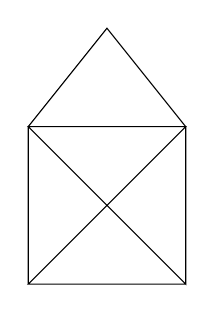
\begin{tikzpicture}
\draw (0,0) -- (0,2) -- (1,3.25) -- (2,2) -- (2,0) -- (0,2) -- (2,2) -- (0,0) -- (2,0);
\end{tikzpicture}
    
	\caption[Mit Tikz programmierte Grafik.]{Mit Tikz programmierte Grafik.}
	\label{fig:tikz_house}
\end{figure}

Ein etwas umfangreicheres Beispiel zur Digitaltechnik ist in Abbildung~\ref{fig:tikz_digital} dargestellt:

\begin{figure}[hbt]
	\centering
	\usetikzlibrary{circuits.logic.US,circuits.logic.IEC}
      \begin{tikzpicture}[circuit logic US]
      \matrix[column sep=7mm]
      {
      \node (i0) {0}; & & \\
      & \node [and gate] (a1) {}; & \\
      \node (i1) {0}; & & \node [or gate] (o) {};\\
      & \node [nand gate] (a2) {}; & \\
      \node (i2) {1}; & & \\
      };
      \draw (i0.east) -- ++(right:3mm) |- (a1.input 1);
      \draw (i1.east) -- ++(right:3mm) |- (a1.input 2);
      \draw (i1.east) -- ++(right:3mm) |- (a2.input 1);
      \draw (i2.east) -- ++(right:3mm) |- (a2.input 2);
      \draw (a1.output) -- ++(right:3mm) |- (o.input 1);
      \draw (a2.output) -- ++(right:3mm) |- (o.input 2);
      \draw (o.output) -- ++(right:3mm) node [right] {$y$ \quad Hier könnte Ihre Formel $y=(0 \land 0) \lor \overline{( 0 \land 1)}$ stehen};
 \end{tikzpicture}

	\caption[Mit Tikz programmierte Grafik, welche bereits vorgefertigte Bibliotheken für Symbole aus der Digitaltechnik nutzt.]{Mit Tikz programmierte Grafik, welche bereits vorgefertigte Bibliotheken für Symbole aus der Digitaltechnik nutzt.}
	\label{fig:tikz_digital}
\end{figure}

%\clearpage

In der Tikz-Umgebung können auch Diagramme mit dem \textit{pgfplot}-Befehlssatz erzeugt werden. In Abbildung \ref{fig:pgfplot} sehen Sie ein Beispiel.

\begin{figure}[hbt]
	\centering
	\begin{tikzpicture}
		\begin{axis}[scale=1.3,legend entries={Messwerte mit Fehlerbalken,
			$\pgfmathprintnumber{\pgfplotstableregressiona} \cdot x  
			\pgfmathprintnumber[print sign]{\pgfplotstableregressionb}$}, legend style={draw=none},legend style={at={(0.01,0.98)},anchor=north west},xlabel=Stromstärke $I \; \mathrm{ \lbrack mA \rbrack}$,ylabel=Spannung $U \; \mathrm{ \lbrack V \rbrack}$]
		\addlegendimage{mark=*,blue}
		\addlegendimage{no markers,red}
\addplot+[error bars/.cd, y dir=both,y explicit]
table[x=x,y=y,y error=errory] 
{pgfplot/messdaten_mitfehler.dat};
\addplot table[mark=none,y={create col/linear regression={y=y}}]
{pgfplot/messdaten_mitfehler.dat};
	\end{axis}
\end{tikzpicture}
	\caption[Diagramm, erstellt mit dem \textit{pgfplot}-Befehlssatz.]{Ein Diagramm, erstellt in der \textit{tikzpicture}-Umgebung mit dem \textit{pgfplot}-Befehlssatz. Das Diagramm stellt Messdaten, deren Fehlerbalken und eine Regressionskurve dar. Die Messdaten werden von einer separaten Datei eingelesen und die Regressionskurve wurde mit \textit{pgfplot} berechnet und erstellt.}
	\label{fig:pgfplot}
\end{figure}

\clearpage

Auch hierzu der Quellcode in Listing~\ref{lst:pgfplot}.

\begin{lstlisting}[caption=Quellcode der Abbildung~\ref{fig:pgfplot}.,label=lst:pgfplot]
\begin{figure}[hbt]
\centering
\begin{tikzpicture}
		\begin{axis}[scale=1.3,legend entries={Messwerte mit Fehlerbalken,
			$\pgfmathprintnumber{\pgfplotstableregressiona} \cdot x  
			\pgfmathprintnumber[print sign]{\pgfplotstableregressionb}$}, legend style={draw=none},legend style={at={(0.01,0.98)},anchor=north west},xlabel=Stromstärke $I \; \mathrm{ \lbrack mA \rbrack}$,ylabel=Spannung $U \; \mathrm{ \lbrack V \rbrack}$]
		\addlegendimage{mark=*,blue}
		\addlegendimage{no markers,red}
\addplot+[error bars/.cd, y dir=both,y explicit]
table[x=x,y=y,y error=errory] 
{pgfplot/messdaten_mitfehler.dat};
\addplot table[mark=none,y={create col/linear regression={y=y}}]
{pgfplot/messdaten_mitfehler.dat};
	\end{axis}
\end{tikzpicture}
\caption[Diagramm, erstellt mit dem \textit{pgfplot}-Befehlssatz.]{Ein Diagramm, erstellt in der \textit{tikzpicture}-Umgebung mit dem \textit{pgfplot}-Befehlssatz. Das Diagramm stellt Messdaten, deren Fehlerbalken und eine Regressionskurve dar. Die Messdaten werden von einer separaten Datei eingelesen und die Regressionskurve wurde mit \textit{pgfplot} berechnet und erstellt.}
\label{fig:pgfplot}
\end{figure}
\end{lstlisting}

In Listing~\ref{lst:tikz} ist der Quellcode der Datei \textit{mess\_fehlerbalken.tex} dargestellt.

\begin{lstlisting}[caption=Quellcode der Datei \textit{mess\_fehlerbalken.tex}.,label=lst:tikz]
\begin{tikzpicture}
\begin{axis}[scale=1.3,legend entries={Messwerte mit Fehlerbalken,
$\pgfmathprintnumber{\pgfplotstableregressiona} \cdot x  
\pgfmathprintnumber[print sign]{\pgfplotstableregressionb}$}, legend style={draw=none},legend style={at={(0.01,0.98)},anchor=north west},xlabel=Stromstärke $I \; \mathrm{ \lbrack mA \rbrack}$,ylabel=Spannung $U \; \mathrm{ \lbrack V \rbrack}$]
\addlegendimage{mark=*,blue}
\addlegendimage{no markers,red}
\addplot+[error bars/.cd, y dir=both,y explicit]
table[x=x,y=y,y error=errory] 
{pgfplot/messdaten_mitfehler.dat};
\addplot table[mark=none,y={create col/linear regression={y=y}}]
{pgfplot/messdaten_mitfehler.dat};
\end{axis}
\end{tikzpicture}
\end{lstlisting}

\clearpage

In Abbildung~\ref{fig:pgfplot2y} wird ein weiters Beispiel für ein Diagramm gezeigt. Oftmals wird eine zweite y-Achse verwendet, um verschiedene Skalen darstellen zu können.

\begin{figure}[hbt]
	\centering
	\begin{tikzpicture}
%
\begin{axis}[
scale=1.3,
ytick pos=left,
xlabel=Zeit $t \; \mathrm{ \lbrack ns \rbrack}$,
ylabel=Spannung $U \; \mathrm{ \lbrack V \rbrack}$
]
\addplot[mark=*,only marks] table[x=x,y=y1] {pgfplot/messdaten_zweiyachsen.dat};
\end{axis}
%
\begin{axis}[
scale = 1.3,
legend style={draw=none},
legend style={at={(0.75,0.6)},
anchor=north west},
axis y line*=right,
axis x line=none,
%ymin=0,
%ymax=100,
ylabel=Strom $I \; \mathrm{ \lbrack mA \rbrack}$
]
\addlegendimage{mark=*,only marks}
\addlegendentry{Spannung}
\addplot[mark=x,only marks,blue] table[x=x,y=y2] {pgfplot/messdaten_zweiyachsen.dat};
\addlegendentry{Strom}
\end{axis}
\end{tikzpicture}
	\caption[Diagramm mit zwei unterschiedlichen y-Achsen.]{Diagramm mit zwei unterschiedlichen y-Achsen.}
	\label{fig:pgfplot2y}
\end{figure}

\clearpage

\subsection{Tabellen}

\begin{table}[hbt]	
	\centering
	\renewcommand{\arraystretch}{1.5}	% Skaliert die Zeilenhöhe der Tabelle
	\captionabove[Liste der verwendeten Messgeräte]{Liste der verwendeten Messgeräte. Die Genauigkeitsangaben beziehen sich auf die Standardabweichung $1\cdot \sigma$.}
	\label{tab:bsp}
	\begin{tabular}{ccccc}
		\textbf{Messgerät} & \textbf{Hersteller} & \textbf{Typ} & \textbf{Verwendung} & \textbf{Genauigkeit}\\ 
		\hline 
		\hline 
		\parbox[t]{0.2\linewidth}{\centering Spannungs-\\versorgung} & Voltmaker & HV2000 & \parbox[t]{0.2\linewidth}{\centering Spannungs-\\versorgung der\\Platine} & $\Delta U = \pm 5 $~mV \\ % Der parbox-Befehl ist erforderlich, damit ein Zeilenumbruch erzeugt werden kann. c-Spalten (zentriert) erlauben nicht automatisch einen Zeilenumpruch. Linksbündig gesetzte p-Spalten erlauben automatisch den Zeilenumbruch.
		Strommessgerät & Currentcount & Hotamp 16 & \parbox[t]{0.2\linewidth}{ \centering Strommessung\\am Versorgungspin\\des µC} & $\Delta I = \pm 0.1$~A \\ 
		\hline 
	\end{tabular} 
\end{table}

Der Quellcode der Beispieltabelle~\ref{tab:bsp} ist in Listing~\ref{lst:tab} zu sehen.

\begin{lstlisting}[caption=Quellcode der Tabelle~\ref{tab:bsp}.,label=lst:tab]
\begin{table}[hbt]	
\centering
\renewcommand{\arraystretch}{1.5}	% Skaliert die Zeilenhöhe der Tabelle
\captionabove[Liste der verwendeten Messgeräte]{Liste der verwendeten Messgeräte. Die Genauigkeitsangaben beziehen sich auf die Standardabweichung $1\cdot \sigma$.}
\label{tab:bsp}
\begin{tabular}{ccccc}
\textbf{Messgerät} & \textbf{Hersteller} & \textbf{Typ} & \textbf{Verwendung} & \textbf{Genauigkeit}\\ 
\hline 
\hline 
\parbox[t]{0.2\linewidth}{\centering Spannungs-\\versorgung} & Voltmaker & HV2000 & \parbox[t]{0.2\linewidth}{\centering Spannungs-\\versorgung der\\Platine} & $\Delta U = \pm 5 $~mV \\ % Der parbox-Befehl ist erforderlich, damit ein Zeilenumbruch erzeugt werden kann. c-Spalten (zentriert) erlauben nicht automatisch einen Zeilenumpruch. Linksbündig gesetzte p-Spalten erlauben automatisch den Zeilenumbruch.
Strommessgerät & Currentcount & Hotamp 16 & \parbox[t]{0.2\linewidth}{ \centering Strommessung\\ am Versorgungspin\\ des \textmu C} & $\Delta I = \pm 0.1$~A \\ 
\hline 
\end{tabular} 
\end{table}
\end{lstlisting}

\clearpage

\subsection{Formeln}

Formeln lassen sich in \LaTeX~ganz einfach schreiben. Es gibt unterschiedliche Umgebungen zum Schreiben von Formeln. Z.~B. direkt im Text $v=s/t$ oder abgesetzt

\[F=m \cdot a\]

oder auch, wie in wissenschaftlichen Dokumenten üblich, nummeriert

\begin{equation}
P=\frac{U^2}{R} \quad .
\label{eqn:leistung}
\end{equation}

Mit einem Label in Formel~\ref{eqn:leistung} lassen sich natürlich auch Formeln im Text referenzieren. \LaTeX~verwendet im Formelmodus einen eigenen Schriftsatz, welcher entsprechend der gängigen Konventionen kursive Zeichen verwendet. Sollen im Formelmodus Einheiten in normaler Schriftart eingefügt werden, dann kann dies über den Befehl \textbackslash \textit{mathrm}\{\} erwirkt werden, wie im Quellcode von Formel~\ref{eqn:leistungMitEinh} zu sehen ist.

\begin{equation}
P=\frac{U^2}{R} = \frac{\left( 100~\mathrm{V}\right)^2}{100~\Omega} = 100~\mathrm{W}\quad .
\label{eqn:leistungMitEinh}
\end{equation}

Zum direkten Vergleich sind die Einheiten in Formel~\ref{eqn:leistungMitEinhfalsch} falsch dargestellt:

\begin{equation}
P=\frac{U^2}{R} = \frac{\left( 100~V\right)^2}{100\,\varOmega} = 100\,W
\label{eqn:leistungMitEinhfalsch}
\end{equation}

Zur einfachen Eingabe von Einheiten kann auch das Package \textbackslash \textit{siunitx} verwendet werden:

\begin{equation}
	P=\SI{100}{\watt}=\SI{100}{\joule\per\second}
\end{equation}

Das sind nur ein paar wenige Beispiele und es gibt sehr viele Packages, um Besonderheiten in Formeln realisieren zu können, z.~B. mehrzeilige Formeln mit vertikaler Ausrichtung. Nennen Sie Formeln nur, wenn diese zum besseren Verständnis auch wirklich nützlich sind.

Folgende Befehle sind innerhalb von Formel-Umgebungen nützlich:
\begin{tabbing}
	\hspace*{0cm} \= \hspace{0.28\linewidth} \= \+\kill
	\textbackslash \textit{text}\{\} oder \textbackslash \textit{mathrm}\{\}	\> Damit kann in Formel-Umgebung Text geschrieben werden.\\ 
	\textbackslash, \textbackslash: \textbackslash; \textbackslash quad \textbackslash qquad \> Zusätzlichen Abstand zwischen Symbolen einfügen.\\
	\textbackslash \textit{notag} \> Nummerierung einer bestimmten Formel ausschalten.
\end{tabbing}

Hier noch ein kleines Beispiel aus der Mathematik:

\begin{equation}
\sum\limits_{n=1}^\infty f\left(x_n\right)\cdot \Delta x=  \lim\limits_{\Delta x \rightarrow 0} \frac{f\left(x_0+\Delta x\right)-f\left(x_0\right)}{\Delta x} = \frac{\diff f}{\diff x} = \dot{f}(x)
\end{equation}

Und abschließend ein Beispiel aus der Physik zum Induktionsgesetz\index{Induktion!Elektromagnetische}:

\begin{equation}
\oint \limits _{\partial {\mathcal {\mathcal {A}}}(t)}{{\vec {E}}\cdot {\text{d}}{\vec {s}}}=-\int \limits _{{\mathcal {A}}(t)}{{\frac {\partial {\vec {B}}}{\partial t}}\cdot {\text{d}}{\vec {A}}}
\end{equation}

		% Zeile auskommentieren bei finalem Dokument!


%\renewcommand{\glossaryname}{Glossar}
%\printglossaries
%\addcontentsline{toc}{chapter}{\glossaryname}

%\renewcommand{\indexname}{Sachwortverzeichnis}
%\printindex								% Erzeugen des Sachwortverzeichnisses

\end{document}